%mainfile: ../master.tex
\chapter{Language}\label{part:design}

This chapter will describe the design of TLDR and explain the reasoning behind the choices made during the design of the language.

The chapter is split into four parts. The first part is the general properties and formal models. This includes the type system, general semantics and scope rules.

After this three sections will cover the specifics of the language. The seperation is between expressions, statements, and actors. Even though actors are also statements, their importance for the characteristics of the language, deemed it worth of a seperate section.

The different sections will contain explanations, which will consist of both formal and informal syntax, semantics and type rulesn of the construct and why this was chosen. Some construct will merit more discussion and explanation than others.

The syntactical constructs will be formally presented with EBNF, but it will be kept close to BNF where it is not deemed that EBNF will provide further clarification. 

To describe the semantics, the formal notation will follow the example set by \cite{huttel2010transitions} for small step semantics. The choice of small step semantics is done, since big step semantics can not describe parallelism, and we did not wish to mix the use of semantics.

In the formal semantic rules have the following convention of what specific symbols are used for:
\begin{itemize}
	\item $n \in Num$ - Numerals
	\item $x \in Sym$ - Symbols
	\item $a \in Aexp$ - Arithmetic expressions
	\item $b \in Bexp$ - Boolean expressions
	\item $S \in Stm$ - Statements	
\end{itemize}

The formal rules have three parts as illustrated in \cref{SS-semantics}

\begin{figure}[H]
\begin{align*}
&\inference[$RULE-NAME$]{[PREMISE]}
                        {[CONCLUSION]}
                        {,[SIDE-CONDITION]}
\end{align*}
\caption{A description of formal small-step semantics}
\label{SS-semantics}
\end{figure}

The conclusion always consists of a transition arrow \enquote{$\Rightarrow$}. On the left hand side the initial code that the rule transitions from and the needed transition functions in their current state inside angel brackets, for example $\Braket{S,env_s,env_a}$. On the right hand side of the transition arrow is the code that this can transition to and the possible updates in the transition functions inside angel brackets, for example $\Braket{S',env_s',env_a'}$. If any symbol are marked with an apostrophe it has the possibility to be something different within the same set. This must be defined in either the premise or side condition.
The premise is how something else must transition before the conclusion can be met. The side condition is for other things that must be true.
The mapping of the transition functions are put inside square brackets, for instance \enquote{$env_s = [x \mapsto \underline{4},y \mapsto \underline{5}]$} denotes that $env_s$ is the transition function where x mapsto the numeral \underline{4} and y to \underline{5}. A transition function can also be expanded using square brackets, for instance we can make a new transition function $env_s'$ that expands on $env_s$ so that it also maps z to the numeral \underline{6}; \enquote{$env_s' = env_s[z \mapsto \underline{6}]$}.

%mainfile: ../master.tex
\section{General Language Properties and Formal Models}
This section will describe the type system of TLDR, the scoping rules and some fundamental semantics for the language.
\jenote{- General typesystem properties
- The semantic model and general constructs}

\subsection{Type System}\label{typesys}

This section first defines what a type system is and presents two categories of type systems. The two type system categories are described and its properties are outlined.

Later in this section, the type system decisions made for TLDR are described, and formal type rules are given.

%\subsection{General Type Systems}

The goal of the type system is to minimise programming errors, while on the other hand not being too restrictive, such that the expressiveness of the language is not reduced. 

\subsubsection{Strictness}
Type systems are often described as \emph{strong} or \emph{weak}. No formal definitions of such categorisations of type systems exist, so this report will use the following understanding of \emph{weak} and \emph{strong} type systems. A type system goes from \emph{weak} to \emph{strong} as the amount of undefined behaviour, unpredictable behaviour or implicit conversions between types approach zero.

\subsubsection{Static Versus Dynamic Type Systems}
Languages can generally be categorised into dynamically typed and statically typed languages. The difference between static and dynamic typing is the time of type checking. In static typing, types are checked at compile time. In dynamic typing, types are checked at run-time.

Statically typed languages have the following advantages over dynamically typed languages.

\begin{itemize}
  \item Type errors are presented at the soonest possible level; compile-time. This makes it impossible to have a program stop unexpectedly because of a type error at run-time
  \item Because of the fact that types are checked at compile time, no overhead is imposed on the compiled program at run-time
\end{itemize}

Of course dynamically typed languages have their uses. One can argue that prototyping a program is done faster in a dynamically typed language because the programmer does not need to think of types when programming. The mental overhead is usually lower. The trade-off of dynamic typing versus static typing is often expressiveness for safety and performance. 

\subsubsection{Type Inference}
Type checking solves the problem of determining if a program is well-typed i.e. does not have any type errors. Type inference can be seen as solving the opposite problem; determine types in a program, making the program well-typed.

In order to reduce the mental overhead and the number of explicit type declarations to write in a language, type inference can be implemented in the compiler. Having types inferred by the compiler in a statically typed language makes the language as expressive as a dynamically typed language, whilst keeping the safety and performance of static typing.

\subsubsection{Summary}
Type systems are defined by the type rules it enforces. Because the strictness of the type rules can vary, type systems can range from being very strict to being very weak.

Generally two different approaches exist to solve the goal of minimising errors in programs. Static typing checks types at compile-time and therefore is able to present type errors at a early stage. Because of this, static typing is often regarded as safer and more performant.

Dynamic typing checks types at run-time and therefore allows the programmer to not have the same mental overhead of thinking about types when programming. \chnote{Kan static typing med type inference ikke også det? Maybe rephrase} This however comes at the price of safety and performance.

Type inference removes the need to explicitly annotate programs with type annotations. This can reduce the mental overhead associated with static typing.

\subsubsection{Type System Choice for TLDR}

The type system for TLDR is \emph{strong} statically typed. No implicit type conversions are made in the type system. This choice of static typing was made based on the domain in which TLDR is meant to be used. Having type errors presented early on in the process of developing programs in the language, means much stronger guarantees can be made about the final running program. This is important because running programs on large systems or distributed systems is costly; whenever a program is run on such systems, the program should produce the expected result without run-time failures.

\subsubsection{Primitive Data Types}
\label{subsec:primitives}

Since mathematics is theoretical abstraction, it is rarely a problem to denote size of numbers, precision on numbers or even infinities. Computers, sadly, have psychical limits which makes it complicated or inefficient to express all these things as just \enquote{numbers}. This the main reason for type declarations on numbers. In mathematics we can also denote a number to be of a certain \enquote{type}, such as the natural numbers, the rational numbers and the real numbers. However in mathematics, this is done for a different reason, namely the different charateristics numbers have.

However, both computer science's type declarations and mathematics' number systems, serve to provide a set of characteristics for the number, and how it will behave. We were inspired by this similarity, and chose to preserve it in our language. However, The mathematical symbol for \enquote{set membership} isn't found on a regular keyboard, so instead we chose the colon \enquote{:}.

When initialising a symbol, it being either mutable or immutable, the programmer must declare its type, as if the symbol belonged to a set, where the set must be a type in our language.

Primitives are the lowest abstraction of value types, that user can interact with, it is not divisible by the user, therefore atomic from their point of view. This means that it is not possible for the user to express any deeping meaning of something being an integer, e.g. an integer composed of 4 bits. %They acts as endpoints of the abstract syntax tree, as it is not possible for the user to express any more descriptive meaning for the compiler.

The following primitives exist in the language. All primitives are lower-cased.

\begin{itemize}
  \item int
  \item real
  \item bool
  \item char
  \item unit
\end{itemize}

\paragraph{Integer}
\label{subsubsec:int}

The integer primitive can have values of whole numbers, e.g. \emph{2}. Integers in TLDR are arbitrary precision, meaning there are no bounds to the range of possible values.

\paragraph{Real}
\label{subsubsec:real}

The real primitive can have values of real numbers. The real primitive's literal representation is as decimal numbers with fractions e.g. \emph{2.5} or \emph{2.0}. As with integers, reals are arbitrary precision.

\paragraph{Bool}
\label{subsubsec:bool}

The bool primitive's value can be either \emph{true} or \emph{false}.

\paragraph{Char}
\label{sec:char}

The char primitive can have values of the ASCII standard. It is written literally as a character defined in the ASCII standard, surrounded by single quotation marks. For example: \emph{ '0' } and \emph{ 'A' }.

\paragraph{Unit}
\label{sec:unit}

The unit primitive can have only one value: itself. The use of the primitive is to signal emptiness.

The prmitives will be exlaborated upon in \cref{operands}.

\subsubsection{Type Declaration}
From the start of the language design, TLDR was supposed to have type inference, due to types not being a known artifact/property in the mathematics of physics and social sciences, which is the scope of the language. Due to prioritisation and time span of the project, it was decided that the language should initially have an explicit type system.

Types not being a known artifact in previously mentioned sciences and mathematics, a technique known from the functional paradigm of separating the type signature from the function definition, as shown here \cref{typesignature}, was chosen. In this signature the function can take any number of arguments and return either a single typed symbol or a new function. The input and output is differenciated by the amount of input parameters (arg1, arg1, ... ,argN) where N would be the amount of inputs and M - N would be the size of the output.

\begin{figure}
\begin{lstlisting}
functionName(arg1, arg2, ... ,argN) :: arg1Type -> arg2Type -> ... -> argMType
\end{lstlisting}
\caption{}
\label{typesignature}
\end{figure}

If the user wants to use functions instead of single typed symbols he or she simply puts these in parentheses as seen in \cref{typesignatureexample0}. Here the function takes another function that maps an integer to an integer and maps this to a real.

\begin{figure}
\begin{lstlisting}
  f(x) : (int -> int) -> real
\end{lstlisting}
\caption{}
\label{typesignatureexample0}
\end{figure}

This can be nested in as many levels as the user desires, as illustrated in \cref{typesignatureexample1}, where the function takes a function typed the same way as in \cref{typesignatureexample0} and maps this to a list of characters. Note that both \cref{typesignatureexample0} and \cref{typesignatureexample1} still only take one argument (x) since this is a function and can be used as such in the body.

\begin{figure}
\begin{lstlisting}
  f(x) : ((int -> int) -> real) -> [char]
\end{lstlisting}
\caption{}
\label{typesignatureexample1}
\end{figure}

\paragraph{Implicit Unit}
This approach posed a problem with the concept of \enquote{unit}. This represents the non-existing value, for the type system. It means that something does not have a value and using it in any context does not make sense. For instance when a function returns unit i.e. nothing, it cannot be assigned to anything. The need for explicitness resides in that The Language Described in This Report has functions as, what is called, \enquote{first class citizens}, meaning that functions can be used as arguments and essentially are treated in the same way as other symbols such as integers, structs etc. Here, the language becomes ambigious with implicit unit, i.e. the user not needing to explicitly tell when a function returns unit. For instance in \cref{typesignatureexample0} the programmer would not be able to tell whether the function takes a function that takes an int and returns an int or returns a function that goes from int to unit since the syntax is the same.
Several proposed solutions will be described here after.

First, a type signature int the language looks as follows:
\begin{verbatim}
  printint(a): int -> int
\end{verbatim}
Where the first $int$ is the parameter $a$ of the function $printint$, and the second $int$ of the signature is the return type.

So in the case that the function $printint$ should not return anything, the last type of the type signature will be decorated with a type of nothing, e.g. unit, as follows:
\begin{verbatim}
  printint(a): int -> unit
\end{verbatim}

The first proposal of a solution is to denote unit as \enquote{nothing}, like this:
\begin{verbatim}
  printint(a): int ->
\end{verbatim}
If the type signature of a function is that it takes nothing as parameter but returns something, like this:
\begin{verbatim}
  printint(): -> int
\end{verbatim}

In the end, it was chosen to explicitly express unit both to avoid confusion for users of the language and since it does not make much sense to focus on improving the explicit type signatures, since type inference is a long term goal for the language. The explicit format ended up as follows:
\begin{verbatim}
  printint(a): int -> unit
\end{verbatim}

\subsubsection{Formal Type Rules}

\begin{align*}
\intertext{The following primitive types are defined}
&\Tpt ::= \Tint \mid \Treal \mid \Tbool \mid \Tchar
\\
\intertext{A tuple is a finite set of ordered elements of arbitrary type $T$}
&\text{TUPLE} ::= T_1 \times T_2 \times \ldots \times T_n
\\            
&\text{B} ::=  \left[ \Tt \right] \mid \Tpt \mid \text{TUPLE} \mid \text{struct<TUPLE>}
\\            
\intertext{All types defined in the type system is defined in $T$.}
&\Tt ::= \text{B} \mid x : B \rightarrow ok
\end{align*}

\subsection{Scoping}

As with most of the choices made during the design of this language, we wanted to strive towards a natural mathematical syntax. This idea was pulling towards the use of linebreaks for denoting the end of a statement, and using indentation for denoting scopes. However since this is impossible to describe with context-free-grammar, and explicitly modifying the parser to support this was adding unnecessarily complexity to the language implementation, we decided upon other constructs.
%impossible - but why?
For denoting scopes we went with the bracket symbols \enquote{\{ \}}. This decision was made due to its similarity with the parentheses know from mathematics, where it has the highest precedence, and also since it is a construct known from many other programming languages. For separating statements, we went with a semi-colon \enquote{;}. This is also a known construct from other programming languages. It is also not in conflict with mathematical use, since there is no widespread consensus of such.


\subsection{Transition System for Formal Semantics}
The transition system used in the formal semantics of TLDR uses four different partial functions. These will be introduced at they are needed but here follows an explanation of each function in succession.
The first transition rule, \enquote{at}, is used to keep track of all actor types. The actor type is a form of prototype used to initialise actors. When created all it statements are run inside a new environment consisting of aEnv, sEnv. This transition rule is the throughout the whole program meaning that all actor types can be initialised everywhere.
\begin{center}
$at = \text{ActorTypes} \rightharpoonup \text{Stm}$
\end{center}
To describe a complete environment in TLDR one needs both the actor environment and the symbol environment. The actor environment is used to keep track of which handles inside an actor that maps to what actor.
\begin{center}
$aEnv = \text{Anames} \rightharpoonup sEnv$
\end{center}
The symbol environment is used to keep track of the which statements and other symbols any symbol maps to. The statements a symbols maps to are the statements are run in an invocation of that symbol, note that all symbols in TLDR are invoked even variables and constants but they will always return the value of which they are assigned, no matter the state af their environment. The symbols that a symbol maps to are used to keep track of what formal parameters an invocation needs, note that this set can be empty.
\begin{center}
$sEnv = \text{Symbols} \rightharpoonup \text{Stm} \times \text{Symbols}$
\end{center}
The last transition rule is used to map to keep track of user structures. These are like actor types in that they maps to the statements that are run to initialise the structure, like a recipe.
\begin{center}
$st = \text{Structs} \rightharpoonup \text{Symbols}$
\end{center}

\subsection{Comments}
\label{subsec:comments}

Comments are declared in C style by \enquote{//} being a single line comment and \enquote{/**/} being a multi line comment.

They follow this grammar:

\kanote{indsæt grammar for kommentar}

A concrete example:

\begin{verbatim}
  // this is a single line comment
  /* this is
     a
     multi line comment */
\end{verbatim}

\section{Expressions}
\label{sec:Expressions}
This part of the language describes expressions. Expressions are in The Language Described in This Report defined as the constructs that have a value. These can be used together with specific operators to create larger expressions as one would do in mathematics. Apart from combining expressions they are often used as the right hand side of an assignment, but can also be used for indexing, the condition in conditional statements, for return values and in general all places where a value is expected.

\subsection{Operators}
First we look at the mathematical operators that can combine expressions.
\setlength{\grammarindent}{100pt}
\begin{grammar}
<Operation> ::= <Operation> <PSIXOPERATOR> <OP6>
 \alt <OP6>

<OP6> ::= <OP6> <PFIVEOPERATOR> <OP5>
 \alt <OP5>

<OP5> ::= <PFOUROPERATOR> <OP5>
 \alt <OP4>

<OP4> ::= <OP4> <PTHREEOPERATOR> <OP3>
 \alt <OP3>

<OP3> ::= <OP3> <PTWOOPERATOR> <OP2>
 \alt <OP2>

<OP2> ::= <OP2> <PONEOPERATOR> <OP1>
 \alt <OP1>

<OP1> ::= <Operand>
 \alt <OP1> <PZEROOPERATOR> <Operand>
 \alt '(' <Operation> ')'

<PZEROOPERATOR> ::= '$\Twedge$' | '\#'

<PONEOPERATOR> ::= '*' | '/' | '\%'

<PTWOOPERATOR> ::= '+' | '-'

<PTHREEOPERATOR> ::= '=' | '!=' | '$\textless$' | '$\textless$=' | '$\textgreater$' | '$\textgreater$='

<PFOUROPERATOR> ::= 'NOT'

<PFIVEOPERATOR> ::= 'AND' | 'NAND'

<PSIXOPERATOR> ::= 'OR' | 'XOR' | 'NOR'
\end{grammar}
The precedence of the operators are created in the grammar. Here the parse tree will be created, such that the $\braket{PSIXOPERATOR}$ is placed highest in the tree and the $\braket{PZEROOPERATOR}$ is placed lowest as standard, meaning that the precedence goes from $\braket{PZEROOPERATOR}$ to $\braket{PSIXOPERATOR}$ with zero having highest precedence. This precedence can be overwritten by parentheses that resets the order so expressions inside parentheses are placed lowest in the tree. All operators have left associativity. An example can be seen in \cref{precedenceExamples} this shows how the parse tree is created from the expression: \\
\begin{center}
$\Tnot a \Tand b \Txor 2 < 3 * (2 + 2) + 4$
\end{center}

\begin{figure}[h]
\centering
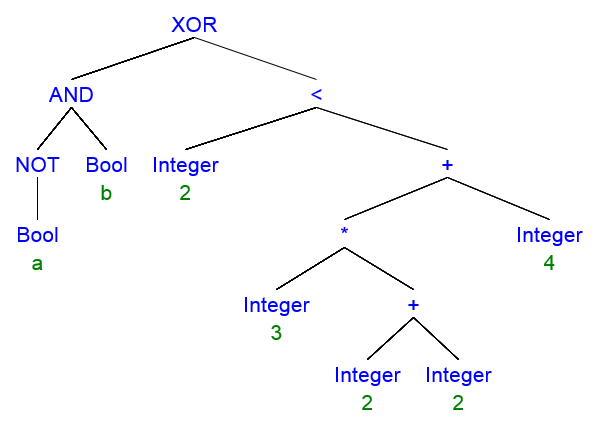
\includegraphics[width=0.7\textwidth]{Design/Expressions/precidenceExamples.png}
\caption{The parse tree for \textnormal{\enquote{$\Tnot a \Tand b \Txor 2 < 3 * (2 + 2) + 4$}}} %[XOR [AND [NOT [Bool a]][Bool b]] [< [Integer 2] [+ [* [Integer 3] [+ [Integer 2] [Integer 2]]] [Integer 4]]]]
\label{precedenceExamples}
\end{figure}

We can see that the operator placed lowest in the tree is \enquote{+} even though \enquote{*} has a higher precedence, and should therefor be lower in the tree. This is done because the parentheses overwrites the the order so that everything inside gets higher precedence as intended. If we insert parentheses to illustrate the implicit precedence in the expression it would look like this:
\begin{center}
$((\Tnot a) \Tand b) \Txor (2 < ((3 * (2 + 2)) + 4))$
\end{center}
In \cref{precedenceExamples} we can see that the \enquote{XOR} operator is placed highest in the tree meaning that it has the lowest precedence. We can also see from the tree that this operator takes the result from \enquote{AND} and \enquote{<} as arguments where \enquote{<} again takes the result from \enquote{+} and the integer 2 as arguments and so on. We can see that the arguments changes type as we traverse the tree. We now look at the semantics and what impact this has on the formal type rules.

\subsubsection{Arithmetic Expressions}

First we look at arithmetic expressions. Arithmetic expressions are in TLDR defined as expressions that evaluates to a number, either a real or integer. The operators that creates the arithmetic expressions are +, -, *, /, \%, $\Tpot$ and \#. The semantics for these operators are as follows:

\begin{itemize}
\item "+" is a binary operator that adds two numbers of the same type

\begin{align*}
&\inference[$\text{ADD}_\text{L}$]{e \vdash a_1 \Rightarrow_A a_1'}
                    {e \vdash  a_1 + a_2 \Rightarrow_A a_1' + a_2}
&
&\inference[$\text{ADD}_\text{R}$]{e \vdash a_1 \Rightarrow_A a_1'}
                    {e \vdash a_2 + a_1 \Rightarrow_A a_2 + a_1'}
\\\\
&\inference[$\text{ADD}_\text{V}$]{}
                    {v_1 + v_2 \Rightarrow_A v}
                    {, v_1 + v_2 = v}
\end{align*}

\item "-" is a binary operator that subtracts two numbers of the same type

\begin{align*}
&\inference[$\text{SUB}_\text{L}$]{e \vdash a_1 \Rightarrow_A a_1'}
                    {e \vdash a_1 - a_2 \Rightarrow_A a_1' - a_2}
&
&\inference[$\text{SUB}_\text{R}$]{e \vdash a_1 \Rightarrow_A a_1'}
                    {e \vdash a_2 - a_1 \Rightarrow_A a_2 - a_1'}
\\\\
&\inference[$\text{SUB}_\text{V}$]{}
                    {v_1 - v_2 \Rightarrow_A v}
                    {, v_1 - v_2 = v}
\end{align*}

\item "*" is a binary operator that multiplies two numbers of the same type

\begin{align*}
&\inference[$\text{MULT}_\text{L}$]{e \vdash a_1 \Rightarrow_A a_1'}
                     {e \vdash a_1 * a_2 \Rightarrow_A a_1' * a_2}
&
&\inference[$\text{MULT}_\text{R}$]{e \vdash a_1 \Rightarrow_A a_1'}
                     {e \vdash a_2 * a_1 \Rightarrow_A a_2 * a_1'}
\\\\
&\inference[$\text{MULT}_\text{V}$]{}
                     {v_1 * v_2 \Rightarrow_A v}
                     {, v_1 * v_2 = v}
\end{align*}

\item "/" is a binary operator that divides two numbers of the same type

\begin{align*}
&\inference[$\text{DIV}_\text{L}$]{e \vdash a_1 \Rightarrow_A a_1'}
                    {e \vdash a_1 / a_2 \Rightarrow_A a_1' / a_2}
&
&\inference[$\text{DIV}_\text{R}$]{e \vdash a_1 \Rightarrow_A a_1'}
                    {e \vdash a_2 / a_1 \Rightarrow_A a_2 / a_1'}
\\\\
&\inference[$\text{DIV}_\text{V}$]{}
                    {v_1 / v_2 \Rightarrow_A v}
                    {, \frac{v_1}{v_2} = v}
\end{align*}

\item "\%" is a binary operator that returns the remainder of a floored division of two numbers of the same type

\begin{align*}
&\inference[$\text{MOD}_\text{L}$]{e \vdash a_1 \Rightarrow_A a_1'}
                    {e \vdash a_1 \% a_2 \Rightarrow_A a_1' \% a_2}
&
&\inference[$\text{MOD}_\text{R}$]{e \vdash a_1 \Rightarrow_A a_1'}
                    {e \vdash a_2 \% a_1 \Rightarrow_A a_2 \% a_1'}
\\\\
&\inference[$\text{MOD}_\text{V}$]{}
                    {v_1 \% v_2 \Rightarrow_A v}
                    {, v_1 \;\; \textrm{mod} \;\; v_2 = v}
\end{align*}

\item "\^{}" is a binary operator that lifts the first number to the power of the second number

\begin{align*}
&\inference[$\text{POW}_\text{L}$]{e \vdash a_1  \Rightarrow_A a_1'}
                    {e \vdash a_1 \Twedge a_2 \Rightarrow_A a_1' \Twedge a_2}
&
&\inference[$\text{POW}_\text{R}$]{e \vdash a_1 \Rightarrow_A a_1'}
                    {e \vdash a_2 \Twedge a_1 \Rightarrow_A a_2 \Twedge a_1'}
\\\\
&\inference[$\text{POW}_\text{V}$]{}
                    {v_1 \Twedge v_2 \Rightarrow_A v}
                    {, v_1 ^ {v_2} = v}
\end{align*}

\item "\#" is a binary operator that roots the first operand to the second operand
\begin{align*}
&\inference[$\text{ROOT}_\text{L}$]{e \vdash a_1 \Rightarrow_A a_1'}
                    {e \vdash a_1 \# a_2 \Rightarrow_A a_1' \# a_2}
&
&\inference[$\text{ROOT}_\text{R}$]{e \vdash a_1 \Rightarrow_A a_1'}
                    {e \vdash a_2 \# a_1 \Rightarrow_A a_2 \# a_1'}
\\\\
&\inference[$\text{ROOT}_\text{V}$]{}
                    {v_1 \# v_2 \Rightarrow_A v}
                    {, \sqrt[v_1]{v_2} = v}
\end{align*}

\item "( )" Parenteses gives what they surrounds the highest precedence.

\begin{align*}
&\inference[$\text{PARENS}_\text{A}$]{e \vdash a_1 \Rightarrow_A a_1'}
                       {e \vdash (a_1) \Rightarrow_A (a_1')}
&
&\inference[$\text{PARENS}_\text{V}$]{}
                       {(v) \Rightarrow_A v}
\end{align*}
\end{itemize}

For simplicity we create the following set since all type rules for these are the same.

\begin{center}
$\Taop = \left\{ {+, -, *, /, \%, \; \Tpot \;} \right\}$
\end{center}

Due to the semantics of all \enquote{AOP} operators these can not evaluate to a real if the two inputs are both integers. Therefore all operators in this set can take either two integers and evaluate to an integer or two reals and evaluate to a real.

The \enquote{\#} operator is a bit different. When taking the an integer root of another integer it can still evaluate to a real, for instance $\sqrt[2]{2}$ evaluates to $1.4142\dots$ Therefore both rules for \enquote{\#} evaluates to a real.

No operator can take a combination of real and integer. This is done since all implicit type casts are avoided in TLDR. The reason for this is that the language is designed to give the programmer all errors as early as possible, preferably on compile-time, see \cref{typesys}. With no implicit type casts the programmer is always aware when type casts are performed and will therefore not be as prone to make runtime type errors.

\begin{align*}
&\inference[$\text{EXPR}_{\Tint,\Tint}$]{\Tenv e_1  : \Tint & 
                       \Tenv e_2 : \Tint}
                    {\Tenv e_1 \mathbin{\text{op}} e_2 : \Tint},  \text{op} \in \Taop
%%%%%%%%%%%%%%%%%%%%%%%%%%%%%%%%%%%%%%%%%%%%%%%%%%%%%%%%%%%%%%%%%%%%%%%%%%%%%%%%%%%%%%%%
\\\\
&\inference[$\text{EXPR}_{\Treal,\Treal}$]{\Tenv e_1 : \Treal & 
                       \Tenv e_2 : \Treal}
                    {\Tenv e_1 \mathbin{\text{op}} e_2 : \Treal},  \text{op} \in \Taop
%%%%%%%%%%%%%%%%%%%%%%%%%%%%%%%%%%%%%%%%%%%%%%%%%%%%%%%%%%%%%%%%%%%%%%%%%%%%%%%%%%%%%%%%
\\\\
&\inference[$\text{ROOT}_{\Tint,\Tint}$]{\Tenv e_1 : \Tint &
                       \Tenv e_2 : \Tint}
                    {\Tenv e_1 \mathbin{\#} e_2 : \Treal}
%%%%%%%%%%%%%%%%%%%%%%%%%%%%%%%%%%%%%%%%%%%%%%%%%%%%%%%%%%%%%%%%%%%%%%%%%%%%%%%%%%%%%%%%
\\\\
&\inference[$\text{ROOT}_{\Treal,\Treal}$]{\Tenv e_1 : \Treal &
                       \Tenv e_2 : \Treal}
                    {\Tenv e_1 \mathbin{\#} e_2 : \Treal}
\end{align*}

\subsubsection{Boolean Expressions}
Boolean expressions are in TLDR defined as expressions that takes boolean types as arguments and returns a boolean type. The boolean expressions can be constructed from the operators AND, NAND, OR, NOR, XOR, NOT.

The following are the semantics for all boolean operators and their truth table.

\begin{itemize}
\item "AND" is a binary operator that returns true if both values are true. False otherwise
\begin{figure}[H]
\centering
  \begin{minipage}[c]{0.45\linewidth}
	  \centering
    \begin{align*}
    &\inference[$\text{AND}_1$]{e \vdash b_1 \Rightarrow_B \bot}
                               {e \vdash b_1 \Tand b_2 \Rightarrow_B \bot}
    \\\\
    &\inference[$\text{AND}_2$]{e \vdash b_1 \Rightarrow_B \top \\ b_2 \Rightarrow_B \bot}
                               {e \vdash b_1 \Tand b_2 \Rightarrow_B \bot}
    \\\\
    &\inference[$\text{AND}_3$]{e \vdash b_1 \Rightarrow_B \top \\ b_2 \Rightarrow_B \top}
                               {e \vdash b_1 \Tand b_2 \Rightarrow_B \top}
    \end{align*}
  \end{minipage}
	\quad
	\begin{minipage}[c]{0.45\linewidth}
	  \centering
    \begin{tabular}{ | c | c | c | }
      \hline
      $e_1$ & $e_2$ & $e_1 \Tand e_2$ \\\hline
      $\bot$ & $\bot$ & $\bot$ \\\hline
      $\bot$ & $\top$ & $\bot$ \\\hline
      $\top$ & $\bot$ & $\bot$ \\\hline
      $\top$ & $\top$ & $\top$ \\\hline
    \end{tabular}
  \end{minipage}
\end{figure}

\item "OR" is a binary operator that returns true if at least one value is true. False otherwise

\begin{align*}
&\inference[OR]{}
                 {e \vdash b_1 \Tor b_2 \Rightarrow_B \Tnot(\Tnot b_1 \Tand \Tnot b_2)}
\end{align*}

\begin{center}
\begin{tabular}{ | c | c | c | }
\hline
$e_1$ & $e_2$ & $e_1 \Tor e_2$ \\\hline
$\bot$ & $\bot$ & $\bot$ \\\hline
$\bot$ & $\top$ & $\top$ \\\hline
$\top$ & $\bot$ & $\top$ \\\hline
$\top$ & $\top$ & $\top$ \\\hline
\end{tabular}
\end{center}

\item "XOR" is a binary operator that returns true if only one operand is true. False otherwise

\begin{align*}
&\inference[XOR]{}
                  {e \vdash b_1 \Txor b_2 \Rightarrow_B (\Tnot(b_1 \Tand b_2)) \Tand (b_1 \Tor b_2)}
\end{align*}

\begin{center}
\begin{tabular}{ | c | c | c | }
\hline
$e_1$ & $e_2$ & $e_1 \Txor e_2$ \\\hline
$\bot$ & $\bot$ & $\bot$ \\\hline
$\bot$ & $\top$ & $\top$ \\\hline
$\top$ & $\bot$ & $\top$ \\\hline
$\top$ & $\top$ & $\bot$ \\\hline
\end{tabular}
\end{center}

\item "NOR" is OR negated.

\begin{align*}
&\inference[NOR]{}
                   {e \vdash b_1 \Tnor b_2 \Rightarrow_B \Tnot( b_1 \Tor b_2 )}
\end{align*}

\begin{center}
\begin{tabular}{ | c | c | c | }
\hline
$e_1$ & $e_2$ & $e_1 \Tnor e_2$ \\\hline
$\bot$ & $\bot$ & $\top$ \\\hline
$\bot$ & $\top$ & $\bot$ \\\hline
$\top$ & $\bot$ & $\bot$ \\\hline
$\top$ & $\top$ & $\bot$ \\\hline
\end{tabular}
\end{center}

\item "NOT" is a unary operator that returns the opposite value of the operand.

\begin{figure}[H]
\centering
\begin{minipage}[c]{0.45\linewidth}
\centering
\begin{align*}
&\inference[$\text{NOT}_\top$]{e \vdash b_1 \Rightarrow_B \top}
                       {e \vdash \Tnot b_1 \Rightarrow_B \bot}
\\\\
&\inference[$\text{NOT}_\bot$]{e \vdash b_1 \Rightarrow_B \bot}
                       {e \vdash \Tnot b_1 \Rightarrow_B \top}
\end{align*}
\end{minipage}
\quad
\begin{minipage}[c]{0.45\linewidth}
\centering
\begin{tabular}{ | c | c | }
\hline
$e_1$ & $ \Tnot e_1$ \\\hline
$\bot$ & $\top$ \\\hline
$\top$ & $\bot$ \\\hline
\end{tabular}
\end{minipage}
\end{figure}

\item "NAND" is a binary operator that returns true if none or a single operand is true. False otherwise.

\begin{align*}
&\inference[NAND]{}
                   {e \vdash b_1 \Tnand b_2 \Rightarrow_B \Tnot( b_1 \Tand b_2 )}
\end{align*}

\begin{center}
\begin{tabular}{ | c | c | c | }
\hline
$e_1$ & $e_2$ & $e_1 \Tnand e_2$ \\\hline
$\bot$ & $\bot$ & $\top$ \\\hline
$\bot$ & $\top$ & $\top$ \\\hline
$\top$ & $\bot$ & $\top$ \\\hline
$\top$ & $\top$ & $\bot$ \\\hline
\end{tabular}
\end{center}
\end{itemize}

All boolean operators, except NOT, takes two booleans and returns a boolean. For the simplicity of the type rules we create the Boolean Operator (BOP):

\begin{center}
$\Tbop = \left\{ {\text{AND, NAND, OR, NOR, XOR}} \right\}$
\end{center}

Note that \enquote{NOT} is not included in the set since it only takes one boolean as input and return a boolean.

\begin{align*}
&\inference[$\text{BOOL}_{BOP}$]{\Tenv e_1 : \Tbool &
                       \Tenv e_2 : \Tbool}
                    {\Tenv e_1 \mathbin{\text{op}} e_2 : \Tbool}, \text{op} \in \Tbop
\\\\
&\inference[$\text{BOOL}_{NOT}$]{\Tenv e : \Tbool}
                    {\Tenv \mathbin{\text{NOT}} \; e : \Tbool}
\end{align*}


\subsubsection{Logical Operations}
\label{sec:logicOps}

Logical operators are in TLDR defined as operators that takes numbers, ie integers and reals, and evaluates to boolean types.

For logical comparisons we chose \enquote{=}. This was done in accordance with the goal of keeping a natural mathematical language. In mathematics \enquote{=} is read as \enquote{is equal to} or simply \enquote{equals}, and is used for stating that two parts are equivalent to each other. Sometimes mathematicians use this statement in a contradicting manner, where they expect to prove the statement to be false. It is from this perspective of being a statement, either true or false, that we chose \enquote{=} to be a logical comparison. The same arguments exist for other types of logical operations.

\begin{itemize}
\item "=" is a binary operator that compares the two operands for equality. Returns true if equal. False otherwise.

\begin{align*}
&\inference[$\text{EQUALS}_\text{L}$]{e \vdash a_1 \Rightarrow_B a_1'}
                    {e \vdash a_1 = a_2 \Rightarrow_B a_1' = a_2}
&
&\inference[$\text{EQUALS}_\text{R}$]{e \vdash a_1 \Rightarrow_B a_1'}
                    {e \vdash a_2 = a_1 \Rightarrow_B a_2 = a_1'}
\\\\
&\inference[$\text{EQUALS}_\text{V1}$]{}
                    {v_1 = v_2 \Rightarrow_B \top}
                    {, v_1 = v_2}
&
&\inference[$\text{EQUALS}_\text{V2}$]{}
                    {v_1 = v_2 \Rightarrow_B \bot}
                    {, v_1 \neq v_2}
\\\\
&\inference[$\text{EQUALS}_\text{Actor}$]{a(act_1) = e\\ a(act_2) = e}
                    {act_1 = act_2 \Rightarrow_B \top}
&
&\inference[$\text{EQUALS}_\text{Actor}$]{a(act_1) = e\\ a(act_2) = e'}
                    {act_1 = act_2 \Rightarrow_B \bot}
                    {e \neq e'}
\end{align*}

\item "!=" is a binary operator that compares the two operands for equality. Returns true if not equal. False otherwise.

\begin{align*}
&\inference[$NEQUALS$]{}
                    {e \vdash a_1 != a_2 \Rightarrow_B \Tnot (a_1 = a_2)}
\end{align*}

\item "<" is a binary operator that compares the two operands. Returns true if the first operand is strictly less than the second operand. False otherwise.

\begin{align*}
&\inference[$\text{LT}_\text{L}$]{e \vdash a_1 \Rightarrow_A a_1'}
                    {e \vdash a_1 < a_2 \Rightarrow_A a_1' < a_2}
&
&\inference[$\text{LT}_\text{R}$]{e \vdash a_1 \Rightarrow_A a_1'}
                    {e \vdash a_2 < a_1 \Rightarrow_A a_2 < a_1'}
\\\\
&\inference[$\text{LT}_\text{V1}$]{}
                    {v_1 < v_2 \Rightarrow_B \top}
                    {, v_1 < v_2}
&
&\inference[$\text{LT}_\text{V2}$]{}
                    {v_1 < v_2 \Rightarrow_B \bot}
                    {, v_1 \geq v_2}
\end{align*}

\item "<=" is a binary operator that compares the two operands. Returns true if the first operand is less than or equal to the second operand. False otherwise.

\begin{align*}
&\inference[$LTEQ$]{}
                    {e \vdash a_1 <= a_2 \Rightarrow_A (a_1 < a_2) \Tor (a_1 = a_2)}
\end{align*}

\item ">" is a binary operator that compares the two operands. Returns true if the first operand is strictly greater than the second operand. False otherwise.

\begin{align*}
&\inference[$\text{GT}_\text{L}$]{e \vdash a_1 \Rightarrow_A a_1'}
                    {e \vdash a_1 > a_2 \Rightarrow_A a_1' > a_2}
&
&\inference[$\text{GT}_\text{R}$]{e \vdash a_1 \Rightarrow_A a_1'}
                    {e \vdash a_2 > a_1 \Rightarrow_A a_2 > a_1'}
\\\\
&\inference[$\text{GT}_\text{V1}$]{}
                    {v_1 > v_2 \Rightarrow_B \top}
                    {, v_1 > v_2}
&
&\inference[$\text{GT}_\text{V2}$]{}
                    {v_1 > v_2 \Rightarrow_B \bot}
                    {, v_1 \leq v_2}
\end{align*}

\item ">=" is a binary operator that compares the two operands. Returns true if the first operand is greater than or equal to the second operand. False otherwise.

\begin{align*}
&\inference[$GTEQ$]{}
                    {e \vdash a_1 >= a_2 \Rightarrow_A (a_1 > a_2) \Tor (a_1 = a_2)}
\end{align*}
\end{itemize}

Since all logical operators take a number and returns a boolean we create the set Logical Operators (LOP):
\begin{center}
$\Tlop = \left\{ {=, !=, <, <=, >, >=} \right\}$	
\end{center}

\begin{align*}
&\inference[$\text{BOOL}_{\Tint,\Tint}$]{\Tenv e_1 : \Tint & 
                       \Tenv e_2 : \Tint}
                    {\Tenv e_1 \mathbin{\text{op}} e_2 : \Tbool}, \text{op} \in \Tlop
\\\\
&\inference[$\text{BOOL}_{\Treal,\Treal}$]{\Tenv e_1 : \Treal &
                       \Tenv e_2 : \Treal}
                    {\Tenv e_1 \mathbin{\text{op}} e_2 : \Tbool}, \text{op} \in \Tlop
\end{align*}

\subsection{Operands}
When creating expressions one also needs operands to use in the operators. The operators are as follows in formal syntax:
\begin{grammar}
<Operand>	::= <Block>
 \alt <Integer>
 \alt <Real>
 \alt <Boolean>
 \alt <Identifier>
 \alt <Literals>
 \alt <Invocation>
\end{grammar}
Some of these operands can evaluate something that is not either an Integer,
\subsubsection{Block}

\begin{grammar}
<Identifier> ::= 'me'
 \alt <Identifier>
 \alt <Identifier> <Accessor>
											
<Identifier> ::= [a-zA-Z][a-zA-Z\_0-9]*-('let' | 'var' | <Primitive> | 'struct' | 'actor' | 'receive' | 'send' | 'spawn' | 'wait' | 'return' | 'for' | 'in' | 'if' | 'else' | 'while' | 'die' | 'me')

<Accessor> ::= '.' <Identifier>
 \alt '.' '[' <Operation> ']'

<Primitive> ::= 'void' | 'int' | 'real' | 'char' | 'bool'

<Literals> ::= <String>
 \alt <ListRange>
 \alt <StructLiteral>
 \alt <Tuple>

<Boolean> ::= 'true' | 'false'

<Integer> ::= '-'?[1-9][0-9]* | '0'

<Real> ::= ([0-9]+'.'[0-9]+)|([0-9]+'.')|('.'([0-9])+)

<String> ::= '\textquotedbl' (U+0020 .. U+007E)* '\textquotedbl'

<Char> ::= '\textquotesingle' U+0020 .. U+007E '\textquotesingle'
\end{grammar}

The following mathematical operations are built into the language. They follow these semantic base rules:

\begin{align*}
&\inference[NUM]{}
                  {e \vdash n \Rightarrow_A v}
                  {, \mathcal{N}(n) = v}
\\\\
&\inference[$\text{INVOKE}_{A1}$]{\Braket{S,e} \Rightarrow_A v}
                  {\Braket{p,e} \Rightarrow_A v}
                  {,e(p) = \Braket{S,\epsilon}}
\\\\
&\inference[$\text{INVOKE}_{A2}$]{\Braket{S_1,e[p_1' \mapsto \Braket{S_2,p_2'}]} \Rightarrow_A v}
                  {\Braket{p_1(p_2),e} \Rightarrow_A v}
                  {,e(p_1) = \Braket{S_1,p_1'}, e(p_2) = \Braket{S_2,p_2'}}
\\\\
\end{align*}


\begin{align*}
&\inference[$\text{INVOKE}_{B1\top}$]{\Braket{S,e} \Rightarrow_B \top}
                  {\Braket{p_1,e} \Rightarrow_B \top}
                  {,e(p) = \Braket{S,\epsilon}}
\\\\
&\inference[$\text{INVOKE}_{B1\bot}$]{\Braket{S,e} \Rightarrow_B \bot}
                  {\Braket{p_1,e} \Rightarrow_B \bot}
                  {,e(p) = \Braket{S,\epsilon}}
\\\\
&\inference[$\text{INVOKE}_{B2\top}$]{\Braket{S_1,e[p_1' \mapsto \Braket{S_2,p_2'}]} \Rightarrow_B \top}
                  {\Braket{p_1(p_2),e} \Rightarrow_B \top}
\\                  
&                 {,e(p_1) = \Braket{S_1,p_1'}, e(p_2) = \Braket{S_2,p_2'}}
\\\\
&\inference[$\text{INVOKE}_{B2\bot}$]{\Braket{S_1,e[p_1' \mapsto \Braket{S_2,p_2'}]} \Rightarrow_B \bot}
                  {\Braket{p_1(p_2),e} \Rightarrow_B \bot}
\\                  
&                 {,e(p_1) = \Braket{S_1,p_1'}, e(p_2) = \Braket{S_2,p_2'}}
\\\\
&\inference[$\text{PARENS}_\text{B}$]{e \vdash b_1 \Rightarrow_B b_1'}
                       {e \vdash (b_1) \Rightarrow_B (b_1')}
\end{align*}

\paragraph{Loop Expressions}
\begin{align*}
\intertext{The conditional body of the while construct must be of type bool. The body of the while-loop can be of any type defined in $\Tt$}
&\inference[WHILE]{\Tenv b : \Tbool &
                  \Tenv e : \Tt}
                 {\Tenv \mathbin{\text{while}} \; (b) \; {e}: ok}
%%%%%%%%%%%%%%%%%%%%%%%%%%%%%%%%%%%%%%%%%%%%%%%%%%%%%%%%%%%%%%%%%%%%%%%%%%%%%%%%%%%%%%%%
\intertext{For loops can only work on lists. The counter variable is the type of a element in the list being iterated.}
&\inference[FOR]{\Tenv l : [\Tpt]}
                 {\Tenv \mathbin{\text{for}} \; \mathbin{\text{x}} \; \mathbin{\text{in}} \; {l} \; : ok },	 \Tenv x : \Tpt
\end{align*}

\paragraph{Comparison of structs}
\begin{align*}
%%%%%%%%%%%%%%%%%%%%%%%%%%%%%%%%%%%%%%%%%%%%%%%%%%%%%%%%%%%%%%%%%%%%%%%%%%%%%%%%%%%%%%%%
\intertext{}
&\inference[STRUCT]{\Tenv e_1: \Tt & \Tenv e_2: \Tt}
                 {\Tenv e_1 = e_2: \Tbool}
\end{align*}

\paragraph{Misc constructs}
\begin{align*}
\intertext{}
&\inference[BLOCK]{\Tenv s_1: \Tt & \Tenv s_2: \Tt'}
                 {\Tenv \{s_1; s_2\} : \Tt'}
%%%%%%%%%%%%%%%%%%%%%%%%%%%%%%%%%%%%%%%%%%%%%%%%%%%%%%%%%%%%%%%%%%%%%%%%%%%%%%%%%%%%%%%%
\intertext{}
&\inference[LET]{}
                 {\Tenv \mathbin{\text{let}} \; e:T: ok}
        %%%%%%%%%%%%%%%%%%%%%%%%%%%%%%%%%%%%%%%%%%%%%%%%%%%%%%%%%%%%%%%%%%%%%%%%%%%%%%%%%%%%%%%%
\intertext{}
&\inference[VAR]{}
                 {\Tenv \mathbin{\text{var}} \; e:T: ok}
                 %%%%%%%%%%%%%%%%%%%%%%%%%%%%%%%%%%%%%%%%%%%%%%%%%%%%%%%%%%%%%%%%%%%%%%%%%%%%%%%%%%%%%%%%
\intertext{}
&\inference[LET1]{\Tenv e_1: \Tt & \Tenv e_2: \Tt}
                 {\Tenv \mathbin{\text{let}} \; e_1 := e_2: ok}
        %%%%%%%%%%%%%%%%%%%%%%%%%%%%%%%%%%%%%%%%%%%%%%%%%%%%%%%%%%%%%%%%%%%%%%%%%%%%%%%%%%%%%%%%
\intertext{}
&\inference[VAR1]{\Tenv e_1: \Tt & \Tenv e_2: \Tt}
                 {\Tenv \mathbin{\text{var}} \; e_1 := e_2: ok}
                        %%%%%%%%%%%%%%%%%%%%%%%%%%%%%%%%%%%%%%%%%%%%%%%%%%%%%%%%%%%%%%%%%%%%%%%%%%%%%%%%%%%%%%%%
\intertext{}
&\inference[NUM]{\Tenv n:\Tint}
                 {\Tenv n: \Tint} 
                        %%%%%%%%%%%%%%%%%%%%%%%%%%%%%%%%%%%%%%%%%%%%%%%%%%%%%%%%%%%%%%%%%%%%%%%%%%%%%%%%%%%%%%%%
\intertext{}
&\inference[NUM1]{\Tenv n_1:\Tint & \Tenv n_2:\Tint}
                 {\Tenv n_1.n_2: \Treal}    
%%%%%%%%%%%%%%%%%%%%%%%%%%%%%%%%%%%%%%%%%%%%%%%%%%%%%%%%%%%%%%%%%%%%%%%%%%%%%%%%%%%%%%%%
\intertext{}
&\inference[INVOKE]{\Tenv n: \Tt}
                 {\Tenv n: \Tt}
\end{align*}

\section{Statements}\label{sec:statements}
Statements are in TLDR defined as constructs that have the possibility to change the state of the program. The state of the program is defined as the symbol by which values are associated. We call this the environment and it is formally described as:
\begin{center}
$e = \text{Symbols} \rightharpoonup \text{Stm} \times \text{Symbols}$
\end{center}
This is a partial function that maps symbols to statements and other statements. These statements are the statements that are run when the symbol is invoked. If these maps to an expression the invocation takes the value of that invocation in the current environment. This can be any expression and as explained the symbol evaluates to whatever the expression maps to. Note that a block is also an expression, see \cref{subsubsec:invocation}. If the statements evaluates only to a statement the symbol is of type \enquote{unit} and it has no value. Note that the statements can still update the state of the program during the invocation. 

If the symbol takes input arguments these are placed inside the \enquote{Symbols} on the right hand side of the arrow. In an invocation these symbols will be mapped to the values given as input parameters.

\subsection{Initialisations}\label{subsec:initialisations}
A new symbol in TLDR can be created via an initialisation. A symbol always maps to at least one statement, i.e. a symbol can not map to nothing. This means that the environment can never map a symbol to the empty set $\epsilon$. For that reason the initialisation always include an assignment with statements and/or expressions. Since symbols only can map to statements a symbol can only have a value when evaluated.

In traditional mathematical notation, the \enquote{=} symbol is also sometimes used to let certain symbols represent a more complex meaning, in order to simplify something, such as an equation or a function. When used like this, often mathematicians put the word \enquote{let} in front of a statement to denote that it is a definition. We wanted to follow this construct as well letting immutable assignment be denoted in this fashion, since they are comparable to definitions. 

But since we wanted assignments, be it mutable or immutable, to have a similarities, we chose \enquote{:=} for all assignments. This concept is less known in traditional mathematics, but is widely used in computational science. In the historically significant languages Fortran and C, the \enquote{=} symbol, was used for this. However, since we wish to keep that symbol closer to its original meaning, we needed something else. \enquote{:=} was chosen, since it is a known symbol from other languages. The asymmetry of the \enquote{:=} symbol also illustrates that it matters which side of the symbol a variable is on, as opposed to the \enquote{=} symbol.

When assigning statements we differentiates between functions and constants/variables. Whether the symbol is constant or not and whether or not it is a function is defined at initialisation. Whether it is a constant or variable binding is denoted with the keywords \enquote{let}, a constant binding, and \enquote{var}, a variable binding. If the statements are bound constant they can never be changed. This is useful, especially in mathematics where many things both functions and constants never changes. But for things like results, state and generic behaviour a variable binding is useful.

Whether a symbol is a function or not is denoted via parentheses, parentheses meaning that it is a function and no parentheses meaning that it is not. Note that a symbol can have empty parentheses and still be a function meaning that there is a difference between \enquote{let a():int := \dots} and \enquote{let a:int := \dots}. The formal syntax is as follows: 

\begin{grammar}
<Initialisation> ::= ('let' | 'var') (<FuncDecl> | <SymDecl>) ':=' <Expression>

<FuncDecl> -> <Identifier> '(' <Ids>? ')' ':' <Types>

<SymDecl> -> <Identifier> ':' <Types>
\end{grammar}
If a symbol is a constant or variable the right hand side of the \enquote{:=} is evaluated and the symbol is assigned the simplest statement that will always evaluate to the value of the evaluation. If the right hand side is evaluated to a number it is formally described as follows:
\begin{align*}
&\inference[$\text{INIT}_{SYM-A1}$]{\Braket{x,env_s} \Rightarrow_A \Braket{x',env_s}}
                         {\Braket{\Tlet \Ta := x,env_s} \Rightarrow_S \Braket{\Tlet \Ta := x',env_s}}
\\\\
&\inference[$\text{INIT}_{SYM-A2}$]{\Braket{x,env_s} \Rightarrow_A v}
                         {\Braket{\Tlet \Tx := x,env_s} \Rightarrow_S env_s'}
\\
&{\Twhere env_s' = env_{s}[\Tx \mapsto \Braket{\{n\},\epsilon}], \mathcal{N}(n) = v}
\end{align*}
The value the expression evaluates is converted via the $\mathcal{N}$ to the numeral and the symbol is assigned this as within a block. In this way an invocation of the symbol will evaluate the block and the same value each time. If the right hand side is evaluated to a boolean the formal semantics are described as follows:
\begin{align*}
&\inference[$\text{INIT}_{SYM-BOOL}$]{\Braket{b,env_s} \Rightarrow_B \Braket{b',env_s}}
                         {\Braket{\Tlet \Ta := b,env_s} \Rightarrow_S \Braket{\Tlet \Ta := b',env_s}}
\\\\
&\inference[$\text{INIT}_{SYM-\top}$]{\Braket{b,env_s} \Rightarrow_B \top}
                         {\Braket{\Tlet \Tx := x,env_s} \Rightarrow_S env_s'}
\\
&{\Twhere env_s' = env_{s}[\Tx \mapsto \Braket{\{\Ttrue\},\epsilon}]}
\\\\
&\inference[$\text{INIT}_{SYM-\bot}$]{\Braket{b,env_s} \Rightarrow_B \bot}
                         {\Braket{\Tlet \Tx := x,env_s} \Rightarrow_S env_s'}
\\
&{\Twhere env_s' = env_{s}[\Tx \mapsto \Braket{\{\Tfalse\},\epsilon}]}
\end{align*}
Again the resulting value is placed as the statement \enquote{true} or \enquote{false} inside a block, thereby always evaluating to this value.

For the representation of functions in our language, we wanted to stay as close as possible to the mathematical functions, such as \enquote{f(x,y) = z}. In order to achieve this, the type of the function arguments had to either be inherent or declared elsewhere. Since we chose to delimit ourselves from type inherence it must be declared. This is done in the same style as any type declaration, with a kolon. Functions in TLDR are treated like values, being reassignable and potentially having a function take another function as a parameter or give it as a return value.

If a symbol is initialised as a function it is dynamically scoped. This means that the statements, a symbol maps to, is evaluated when it is invoked, in the environment in which it is invoked, meaning that if the function is impure, see \cref{subsubsec:invocation}, it will use the statements the symbols maps to at the time of invocation not initialisation. This means that a function when not invoked maps to the statements it was assigned and other functions can be assigned these or use them as inputs.

\begin{align*}
&\inference[$\text{INIT}_{FUNC1}$]{}
                         {\Braket{\Tlet \Tx() := \{S\},sEnv} \Rightarrow_S sEnv'}
												 {, sEnv' = sEnv[\Tx \mapsto \Braket{S,\epsilon}]}
\end{align*}
If the symbol is a function and takes input parameters these are placed as formal parameters in the symbols ordered set the symbol maps to in the order they appear.
\begin{align*}
&\inference[$\text{INIT}_{FUNC2}$]{}
                         {\Braket{\Tlet \Tx(x) := \{S\},sEnv} \Rightarrow_S sEnv'}
												 {, sEnv' = sEnv[\Tx \mapsto \Braket{S,y}]}
\end{align*}
Expanding the amount of input parameters is a trivial task. All symbols are placed in the set in the order they appeal in the code. 
\begin{align*}
&\inference[$\text{INIT}_{FUNC3}$]{}
                         {\Braket{\Tlet \Tx(x,y) := \{S\};,sEnv} \Rightarrow_S sEnv'}
												 {, sEnv' = sEnv[\Tx \mapsto \Braket{S,\{x,y\}}]}
\end{align*}
Note that all rules are defined as constant bindings (\enquote{let}) but the exact same semantic goes for all variable bindings, since the allowance of reassignment is checked by the type system.

\begin{grammar}
<Identifier> ::= 'me'
 \alt <Id>
 \alt <Id> <Accessor>

<Id> ::= [a-zA-Z][a-zA-Z\_0-9]*-('let' | 'var' | 'int' | 'real' | 'char' | 'bool' | 'struct' | 'actor' | 'receive' | 'send' | 'spawn' | 'return' | 'for' | 'in' | 'if' | 'else' | 'while' | 'die' | 'me ')

<Ids> ::= <Identifier> (',' <Identifier>)*

<Types> ::= <Type> ('->' <Type>)*

<Type> ::= <PrimitiveType>
 \alt <Identifier>
 \alt <ListType>
 \alt <TupleType>

<TupleType> ::= '(' <Types> ')'

<ListType> ::= '\{' <Types> '\}'

<PrimitiveType> ::= 'int' | 'real' | 'char' | 'bool'
\end{grammar}

As can be seen, values can either be an immutable constant, or a muteable variable.

A constant binding can never have its value changed. For example, if \enquote{a} is bound to \enquote{5}, \enquote{a} can never refer to another value than \enquote{5} in the same lexical scope. 

The syntax for constant value assignment is as follows.
\begin{verbatim}
  let <symbolName> : <type> := <value>
\end{verbatim}
A concrete example:

\begin{verbatim}
  let x : int := 2
\end{verbatim}

A variable binding can always change the value it refers to. For example, if \enquote{b} is bound to \enquote{2}, it is perfectly possible to later in the source code refer to {10}.

The syntax for variable value assignment is as follows.

\begin{verbatim}
  var <symbolName> : <type> := <value>

// a later reassignment
  <symbolName> := <value>
\end{verbatim}
A concrete example:

\begin{verbatim}
  var a : int := 2
  
// a later reassignment
  a := 2
\end{verbatim}

\subsection{Assignment}\label{subsec:assignment}
\begin{align*}
&\inference[ASS]{\Braket{S,e} \Rightarrow_S \Braket{S',e'}}
                 {\Braket{\Tx := S,e} \Rightarrow_S \Braket{\Tx := S',e'}}
\\\\
&\inference[ASS]{\Braket{S,e} \Rightarrow_S v}
                 {\Braket{\Tx := S,e} \Rightarrow_S e'}
								 {, e' = e[\Tx \mapsto \Braket{\{n\},\epsilon}], \mathcal{N}(n) = v}
\end{align*}


\begin{align*}
\intertext{}
&\inference[LET]{}
                 {\Tenv \mathbin{\text{let}} \; e:T: ok}
\\\\
&\inference[VAR]{}
                 {\Tenv \mathbin{\text{var}} \; e:T: ok}
\\\\
&\inference[LET1]{\Tenv e_1: \Tt & \Tenv e_2: \Tt}
                 {\Tenv \mathbin{\text{let}} \; e_1 := e_2: ok}
\\\\
&\inference[VAR1]{\Tenv e_1: \Tt & \Tenv e_2: \Tt}
                 {\Tenv \mathbin{\text{var}} \; e_1 := e_2: ok}
\end{align*}

\subsubsection{Functions}
\label{subsec:functions}

Functions can be declared in two ways. By separating the type signature and the function body or by combining the signature and the function body.

\paragraph{Separated function declaration}

The syntax for the separated function declaration is as follows. The type signature and the body must be declared in the same lexical scope.

\begin{verbatim}
  <funcName> : <typeSignature>;
  let <funcName>(<parameterList>) := {<body>};
\end{verbatim}

A concrete example:

\begin{verbatim}
  plus : int -> int -> Int;
  let plus(x, y) := {x + y};
\end{verbatim}


\paragraph{Combined function declaration}

The syntax for the combined function declaration is as follows.

\begin{verbatim}
  let <funcName>(<parameterList>) : <typeSignature> := {<body>};
\end{verbatim}

A concrete example:

\begin{verbatim}
  let plus(x, y) : Int -> Int -> Int := {x + y};
\end{verbatim}

%mainfile: ../../master.tex
\subsection{Structures}
\label{subsec:structs}

In TLDR there are three ways to do encapsulation. Actors, Tuples and structs. Structs are unique by being fully accessible within the scope, and having named fields. Structs are especially useful in TLDR for creating messages.

\subsubsection{Defining Structures}
\label{sec:defStructures}

\subsubsection{Syntax}

Structures are defined by using the \enquote{struct} keyword. The grammar for declaring structs are as follows:

\begin{grammar}
  <Struct> ::= 'struct' <Identifier> ':= \{' <TypeDecls> '\}'
\end{grammar}

And a concrete example:

\begin{lstlisting}[style=TLDR]
  struct Person := {Name:[char]; Age:int}
\end{lstlisting}

\subsubsection{Semantics}

having these semantics:

\begin{align*}
\intertext{In the case that we have multiple S of assignments, we can rewrite the T to now map to new s' that includes x, in the new st' environment and the rest of declaration statements}
&\inference[$\text{STRUCT}$]{}
                            {\Braket{\Tstruct T := \{x:T';S\}, env_s, st} \Rightarrow_S \Braket{\Tstruct T := \{S\},env_s,st'}}
\\
&{\Twhere st' = st[T \mapsto s'],st(T) = s,s' = s \cup x]}
\\\\
\intertext{In the case that we have multiple S of assignments, we can rewrite the T to now map to new s' that includes x, in the new st' environment}
&\inference[$\text{STRUCT}$]{}
                            {\Braket{\Tstruct T := \{x:T\}, env_s, st} \Rightarrow_S \Braket{env_s,st'}}
\\
&{\Twhere st' = st[T \mapsto s'],st(T) = s,s' = s \cup x]}
\end{align*}

\begin{align*}
&\inference[$\text{STRUCT}$]{}
                            {\Braket{\Tstruct T_1 := (x:T_2;S), env_s} \Rightarrow_S \Braket{\Tstruct T_1 := (S),env_s'}}
\\
&{\Twhere env_s' = env_s[T \mapsto \Braket{\epsilon,s'}],env_s(T) = s,s' = s \cup x}
\\\\
&\inference[$\text{STRUCT}$]{}
                            {\Braket{\Tlet \; \Ta:T := (S),env_s} \Rightarrow_S \Braket{\Ta := (S),env_s'}}
\\
&{env_s' = env_s[x \mapsto (S,s)],env_s(T) = (\epsilon,s)]}
\\\\
&\inference[$\text{STRUCT}$]{\Braket{x,sEnv} \Rightarrow_a \Braket{x',sEnv}}
                            {\Braket{\Tlet \Ta := (f := x;S),env_s} \Rightarrow_S \Braket{\Tlet \Ta := (f := x';S),env_s}}
\\\\
&\inference[$\text{STRUCT}$]{\Braket{x,sEnv} \Rightarrow_a n}
                            {\Braket{\Tlet \Ta := (f := x;S),env_s} \Rightarrow_S \Braket{\Tlet \Ta := (S),env_s[s.f \mapsto {n}]}}
\\\\
&\inference[$\text{STRUCT}$]{sEnv(x) = \Braket{(S),s}}
                            {\Braket{\Tlet \Ta := (f := x;S),env_s} \Rightarrow_S \Braket{\Tlet \Ta.f.s := s;\Ta := (S),env_s}}
\\\\
&\inference[$\text{STRUCT}$]{\Braket{x,sEnv} \Rightarrow_a n}
                            {\Braket{\Tlet \Ta := (f := x;S),env_s} \Rightarrow_S \Braket{\Tlet s := (S),env_s[s.f \mapsto {n}]}}
\\\\
&\inference[$\text{LIST}$]{}
                            {\Braket{s:[T] := [x_n,..,x_m],sEnv_1} \Rightarrow_S \Braket{s:[T] := [x_{n+1},..,x_m],sEnv_1}}
\\
&{sEnv_1(s) = \Braket{\epsilon,\epsilon,sEnv_2},sEnv_2' = sEnv_2[n \mapsto x_n],sEnv_1'(s) = \Braket{\epsilon,\epsilon,sEnv_2'}}
\\\\
&\inference[$\text{TUPLE}$]{}
                           {\Braket{s:[T] := [x_n,..,x_m],sEnv_1} \Rightarrow_S \Braket{s:[T] := [x_{n+1},..,x_m],sEnv_1}}
\\
&{sEnv_1(s) = \Braket{\epsilon,\epsilon,sEnv_2},sEnv_2' = sEnv_2[n \mapsto x_n],sEnv_1'(s) = \Braket{\epsilon,\epsilon,sEnv_2'}}
\end{align*}

\subsubsection{Type Rules}

\begin{align*}
\intertext{The elements can be of any type defined in $\Tt$}
&\inference[STRUCT]{E[s \mapsto (e_1:\Tt_1;e_2:\Tt_2;...;e_n:\Tt_n) \rightarrow ok]\vdash S : ok & }
                 {\Tenv \mathbin{\text{struct s}} := \{e_1:\Tt_1;e_2:\Tt_2;...;e_n:\Tt_n\}; S: ok}
\end{align*}



\subsubsection{Initialising Structures}
\label{sec:initStructures}

Structs can be initialised and assigned to symbols using either a constant assignment or a variable assignment. Structs initialised as a constant assignment cannot change any of the fields of the structs; the struct is immutable. Structs initialised as a variable assignment can change all of its fields at any time; the struct is mutable.

\subsubsection{Syntax}

The syntax for initialising a struct is as follow.

\begin{grammar}
<StructLiteral> ::= '(' (<Reassignment>';')* ')' (':' <Identifier>)?
\end{grammar}


With concrete examples for immutables:

\begin{verbatim}
  let Alice:Person := (Name := "Alice"; Age := 20);
\end{verbatim}

And for mutable struct is as follow.

\begin{verbatim}
  var Alice:Person := (Name := "Alice"; Age := 20);
\end{verbatim}

And for usage in lists.

\begin{verbatim}
  [(Name := "Alice"; Age := 20):Person];
\end{verbatim}

\subsubsection{Access to Structure Fields}
\label{sec:accessStructFields}

Fields can be access using the following syntax.

\begin{verbatim}
  Alice.Name; // "Alice"
\end{verbatim}

Structs declared as mutable can have fields reassigned using the following syntax.

\begin{verbatim}
  Alice.Name; // "Alice"
  Alice.Name := "Bob";
  Alice.Name; // "Bob";
\end{verbatim}
 
\subsubsection{Semantics}

\begin{align*}
\intertext{In the case that we have multiple S of assignments, we can rewrite the s to now having an accessor that maps to value of the first assignment and the rest of pending assignments in s}
&\inference[$\text{STRUCT}$]{}
                            {\Braket{\Tlet \; s:T := (f := x;S),env_s,st} \Rightarrow_S \Braket{s.f := x;\Tlet \; s:T := (S),env_s,st}}
\\\\
\intertext{In the case that we have only one assignment, we can rewrite the s to now having an accessor that maps to value of the assignment}
&\inference[$\text{STRUCT}$]{}
                            {\Braket{\Tlet \; s:T := (f := x),env_s,st} \Rightarrow_S \Braket{s.f := x,env_s,st}}
%\\\\
%&\inference[$\text{STRUCT}$]{}
%                            {\Braket{(f := x;S),env_s,st} \Rightarrow_S \Braket{s.f := x;\Tlet \; s:T := (S),env_s,st}}
%\\\\
%&\inference[$\text{STRUCT}$]{}
%                            {\Braket{(f := x):T,env_s,st} \Rightarrow_S \Braket{s.f := x,env_s,st}}
\end{align*}

\subsubsection{Type Rules}

Each e of type t is matching the declared struct types, evaluates to the type of the declared struct.

\begin{align*}
&\inference[STRUCTLITERAL]{\Tenv (e_1 : \Tt_1;e_2 : \Tt_2;...;e_n : \Tt_n):\Tt'}
                 {\Tenv \mathbin{\text{(}} e_1; e_2;...;e_n\mathbin{\text{)}}:\Tt': \Tt'}
\end{align*}

\subsubsection{Comparison of Structs}
\begin{align*}
&\inference[STRUCT]{\Tenv e_1: \Tt & \Tenv e_2: \Tt}
                 {\Tenv e_1 = e_2: \Tbool}
\end{align*}

\subsubsection{For-loop Statements}
\label{subsec:forLoopStatements}

A for-loop iterates through a list of elements.

The for loop statement has the following syntax.

\begin{verbatim}
  for <element> in <collection> {<loopBody>}
\end{verbatim}

A concrete example:

\begin{verbatim}
  for i:int in [0..10]:[int] { /* Do stuff with i elements */ }
\end{verbatim}
\subsubsection{While-loop Statements}
\label{subsec:whileLoopStatements}

The while loop statement runs a block of statements until a boolean expression returns false.

\paragraph{While loop}
\label{sec:whileLoop}

The while statement has the following syntax.

\begin{verbatim}
  while (<boolExp>) {<loopBody>}
\end{verbatim}

A concrete example:

\begin{verbatim}
  var i:int := 0;
  while (i < 10) {i := i + 1}
\end{verbatim}

\subsubsection{Semantics}

\begin{align*}
&\inference[$\text{WHILE}_\top$]{e \vdash b \Rightarrow_B \top}
                       {\Braket{\Twhile(b)\{S\},e} \Rightarrow_S \Braket{\{S\}; \Twhile (b)\{S\},e}}
\\\\
&\inference[$\text{WHILE}_\bot$]{e \vdash b \Rightarrow_B \bot}
                       {\Braket{\Twhile(b)\{S\},e} \Rightarrow_S e}
\end{align*}
%mainfile: ../master.tex
\subsection{If-statements}
\label{subsec:ifStatements}

If-statements can be written either as a if-else statement or just as an if-statement. In an if-else statement, the body just after the condition is evaluated if the condition evaluates to the boolean value \emph{true}. If the condition evaluates to \emph{false}, the body after the else keyword is evaluated. In an if-statement, the body after the condition is run, if the condition has the value \emph{true}. If the condition has value \emph{false}, nothing is evaluated.

\subsubsection{Syntax}

\begin{grammar}
<If> ::= 'if' <Expression> <Block>

<IfElse> ::= 'if' <Expression> <Block> 'else' <Block>
\end{grammar}

A concrete example:

\begin{verbatim}
  // if-then-else statement
  if (2 + 2 = 4) {"math works!"}
  else {"something is wrong here!"}

  // if-statement
  if (remainingTime < 10) {initiateCountdown()}
\end{verbatim}

\subsubsection{Semantics}

\begin{align*}
\intertext{In the case that the condition $b$ is true, the rule for the if-statement can simply be rewritten to the statement $S$.}
&\inference[$\text{IF}_\top$]{}
                      {\Braket{if(b)\{S\},sEnv} \Rightarrow_S \Braket{\{S\},sEnv}}
                      {,b \Rightarrow_B \top}
\\\\
\intertext{In the case that the condition $b$ is false, nothing is evaluated, and the if-statement is rewritten to the symbol environment $sEnv$.}
&\inference[$\text{IF}_\bot$]{}
                      {\Braket{if(b)\{S\},sEnv} \Rightarrow_S sEnv}
                      {,b \Rightarrow_B \bot}
\\\\
\intertext{In the case that the condition $b$ is true, the rule for the if-else statement is rewritten to $S_1$.}
&\inference[$\text{IF-ELSE}_\top$]{}
                      {\Braket{if(b)\{S_1\}else\{S_2\},e} \Rightarrow_S \Braket{\{S_1\},e}}
                      {,b \Rightarrow_B \top}
\\\\
\intertext{In the case that the condition $b$ is false, the rule can be rewritten to $S_2$.}
&\inference[$\text{IF-ELSE}_\bot$]{}
                      {\Braket{if(b)\{S_1\}else\{S_2\},e} \Rightarrow_S \Braket{\{S_2\},e}}
                      {,b \Rightarrow_B \bot}
\end{align*}

\subsubsection{Type Rules}

\begin{align*}
\intertext{The conditional body of a if-statement must be of type bool. The body can be of any type defined in $\Tt$. The type of the if-statement is well-typed.}
&\inference[$\text{IF}$]{\Tenv b : \Tbool &
                  \Tenv e : \Tt}
                 {\Tenv \mathbin{\text{if}} \; (b) \; \{e\}: ok}
%%%%%%%%%%%%%%%%%%%%%%%%%%%%%%%%%%%%%%%%%%%%%%%%%%%%%%%%%%%%%%%%%%%%%%%%%%%%%%%%%%%%%%%%
\intertext{The conditional body of a if-else-statement must be of type bool. The two bodies can be of any type defined in $\Tt$. The type of the if-else-statement is well-typed.}
&\inference[$\text{IF-ELSE}$]{\Tenv b : \Tbool &
                  \Tenv e_1 : \Tt &
                  \Tenv e_2 : \Tt}
                 {\Tenv \mathbin{\text{if}} \; (b) \; \{e_1\} \mathbin{\text{else}} \{e_2\}: ok}
\end{align*}

\subsection{Match Statements}
\label{subsec:matchStatements}

Match statements can be seen as syntactical sugar for multiple chained if-statements. The syntax is as follows.

\begin{verbatim}
  match <whatToMatchOn> {
    <case1> -> <actionOnCase1>
    <case2> -> <actionOnCase2>
    ...
    <caseN> -> <actionOnCaseN>
  }
\end{verbatim}

A concrete example:

\begin{verbatim}
  match (1, 2) {
    (0, n) -> // this case will never be reached
    (1, n) -> print("Case reached!");
    _ -> // default case that matches everything
  }
\end{verbatim}

\subsubsection{Delimitation}

Due to other work being deemed more importantly, match-statements will not be further developed. A future improvement to TLDR could possibly include match statements.

\section{Actors}

Here follows descriptions of the usage of actors in TLDR. This includes different principles, functionalities, syntactical and the semantics. But before we can discuss the use of actors in TLDR, we must first cover the semantics of the parallelism used.

\subsubsection{Semantics of parallelism}

\kanote{forklaring af parallisms semantic}

\begin{align*}
%%%%%%%%%%%%%%%%%%%%%%%%%%%%%%%%%%%%%%%%%%%%%%%%%%%%%%%%%%%%%%%
\intertext{The left side of a parallel statement is executed, but not finished. The environment and actor model is updated when executing $S_1$.}
&\inference[$\text{PAR}_1$]{\Braket{S_1,e_1,\Ta} \Rightarrow_S \Braket{S_1',e_1',\Ta'}} 
                           {\Braket{S_1,e_1,\Ta}|\Braket{S_2,e_2,\Ta} \Rightarrow_S \Braket{S_1',e_1',\Ta'}|\Braket{S_2,e_2,\Ta'}}
%%%%%%%%%%%%%%%%%%%%%%%%%%%%%%%%%%%%%%%%%%%%%%%%%%%%%%%%%%%%%%%
\intertext{The left side of a parallel statement is executed, and finishes. The environment and actor model is updated when executing $S_1$.}
&\inference[$\text{PAR}_2$]{\Braket{S_1,e_1,\Ta} \Rightarrow_S \Braket{e_1',\Ta'}} 
                           {\Braket{S_1,e_1,\Ta}|\Braket{S_2,e_2,\Ta} \Rightarrow_S \Braket{S_2,e_2,\Ta'}}
%%%%%%%%%%%%%%%%%%%%%%%%%%%%%%%%%%%%%%%%%%%%%%%%%%%%%%%%%%%%%%%
\intertext{The right side of a parallel statement is executed, but not finished. The environment and actor model is updated when executing $S_2$.}
&\inference[$\text{PAR}_3$]{\Braket{S_2,e_2,\Ta} \Rightarrow_S \Braket{S_2',e_2',\Ta'}} 
                           {\Braket{S_1,e_1,\Ta}|\Braket{S_2,e_2,\Ta} \Rightarrow_S \Braket{S_1,e_1,\Ta'}|\Braket{S_2',e_2',\Ta'}}
%%%%%%%%%%%%%%%%%%%%%%%%%%%%%%%%%%%%%%%%%%%%%%%%%%%%%%%%%%%%%%%
\intertext{The right side of a parallel statement is executed, and finishes. The environment and actor model is updated when executing $S_2$.}
&\inference[$\text{PAR}_4$]{\Braket{S_2,e_2,\Ta} \Rightarrow_S \Braket{e_2',\Ta'}}
                           {\Braket{S_1,e_1,\Ta}|\Braket{S_2,e_2,\Ta} \Rightarrow_S \Braket{S_1,e_1,\Ta'}}
%%%%%%%%%%%%%%%%%%%%%%%%%%%%%%%%%%%%%%%%%%%%%%%%%%%%%%%%%%%%%%%
\end{align*}

\subsubsection{Isolation and Independence}

A central principle in TLDR is the use of actors, based on the actor model. Actors are to be seen as entities with interaction. In other words, in order for a construct to qualify as an actor, it must define a way to behave when other actors interact with it. Actors should function independently, and in that regard, not be open to direct manipulation and only able to be changed through the messages it receives. This requirement is due to the wish of separation of processes, which will allow for greater concurrency by letting processes operate on local data instead of global, shared data. Therefore, TLDR tries to encourage natural isolation of functionality through actors, which in turn will also give a greater control of race conditions as no data is ever accessed by more than one process.

\subsubsection{The Main Actor}

Main is always the first actor, and any program writtin in TLDR is started with main receiving the arguments message. This is done to force the programmer to start and end the program with an actor, which will better support the actor modeling perspective. This means that the main actor is started with a message for the arguments, and when the main actor is killed the program will stop executing, whether or not there are still working actors.

The argument message called args, is a struct which consists of a argument counter called argv, and a lists of char lists called argv.

Another way that this affects the programmer, is the idea of spawning actors and having them send messages to main, instead of calling functions and having them return. This also means that there must be a way to reference main, since it is not spawned by another actor. This is solved by the introduction of the \enquote{me} keyword, which will evaluate to a reference to the current actor. This is very useful, especially if an actor wishes to delegate work to other actors. The message that is sent with the work, must simply contain a reference back to the delegating actor, which was included through the use of the \enquote{me} keyword.

Here are the semantics for the main actor.

\begin{align*}
&\inference[$\text{MAIN}$]{input \mapsto \Braket{S,\epsilon}}
                          {\Braket{\Treceive \Tr:args := \{S\},e} \Rightarrow_S \Braket{\Tr := input;S, e]}}
\end{align*}

\subsubsection{Construction of an Actor}
\label{sub:constructionOfAnActor}

The syntactical declaration of an actor is as follows:

\begin{lstlisting}
actor <identifier> := {
  <functionality>
}
\end{lstlisting}

And a concrete example could be:

\begin{verbatim}
  actor earth := {
    var temperature:real := 0;
    receive sunlight:light := {
      temperature := temperature + 0.1;
    }
  }
\end{verbatim}

As shown, the actor keyword precedes the definition, denoting the meaning of said definition. After the keyword an identifier of the declaration is needed, which will serve as the specific actor type. It is suggested that this identifier reflects the role of the actor in a context of use. Noticeably there is no \enquote{let} or \enquote{var} keyword in front of the definition, as there usually is when assigning. This is a deliberate choice since \enquote{let} and \enquote{var} implies interchangeability, which is not an option is this case. If variable declaration of actor definitions were possible, it would effectively be the equivalent of changing the definition of a type on run-time, which would make little sense, and completely undermine the type safety in the language.

Some general semantics of actors:

\begin{align*}
&\inference[TYPEOF]{}
                  {e \vdash m \Rightarrow_T t}
                  {, \mathbb{T}(m) = t}
\\\\
&\inference[$\text{ACTOR}$]{a' = a[\Tact \mapsto e \times st]}
                           {\Braket{\Tactor \Tact := \{S\}, a} \Rightarrow_S \Braket{S,e,at[\Tact \mapsto S],a'}}
\\\\
&\inference[$\text{ACTOR}$]{}
                           {\Braket{\Tactor \Tact := 1S, at} \Rightarrow_S \Braket{at[\Tact \mapsto S]}}
\end{align*}

\subsubsection{Basic Actor Functionality}
\label{subsubsec:BasicActorFunctionality}
There are four basic functionalities for actors: \enquote{spawn}, \enquote{die}, \enquote{send}, and \enquote{receive}, which are all used through keywords. It was desired to keep the syntax of these functionalities different from the syntax of functions. Even though they behave much like functions, taking input and giving output, they are more powerful. For example, regular functions cannot contain a type as a parameter, but the \enquote{spawn} functionality does this. Due to this and more differences, which follow below, it was decided to separate them syntactically.

The \enquote{spawn} functionality is used to create new instances of actors. And example could be:

\label{actorfuncSpawn}
\begin{lstlisting}
actor <identifier> := {
 <functionality>
}

let MyActor:<identifier> := spawn <identifier> <message>;

or alternatively:

var MyActor:<identifier> := spawn <identifier> <message>;
\end{lstlisting}

As can be seen above, there are four parts of the spawn functionality: an identifier, the keyword, the type of the actor, and optionally an initial message. Firstly, the identifier is preceded by a keyword for mutability, such as \enquote{let} or \enquote{var}. This allows for the substitution of handles, which provides possibilities of dynamic changes. This however opens up the possibility of \enquote{losing contact} with an actor, if the handle is replaced. This could potentially lead to memory leaks if not handled properly. \kanote{reference til garbage collection afsnit}

When spawning a new actor, you can also choose to add a message. The reason for this is to give the programmer a way of initialising the new actor with a certain message. In object-oriented languages this is usually done with a constructor, however doing it via a constructor would conflict with a central principle, since it would mean manipulating an actors state directly.

The semantics of \enquote{spawn} is as follows:

\begin{align*}
&\inference[$\text{SPAWN}$]{}
                       {\Braket{\Tlet \Tact:T := \Tspawn \; T \Tm,\Ta} \Rightarrow_S \Braket{\Tsend \Tact \Tm,\Ta[act \mapsto e \times st]}}
\\
&                       {, \Ta(x) \mapsto \Braket{S,p} , \Ta' = \Ta[\Tact \mapsto \Braket{S, p}]}
\end{align*}

Type rules for \enquote{spawn}:

\begin{align*}
\intertext{}
&\inference[SPAWN]{}
                 {\Tenv \mathbin{\text{spawn}} \; \Tt: \Tt}
\end{align*}

After an actor has been spawned, it will be possible to send messages to it. This is done with the \enquote{send}-keyword. This can be done as follows:

\label{actorfuncSend}
\begin{lstlisting}
MyMsg:int := 42;

Send MyActor MyMsg;
\end{lstlisting}

It is also possible for actors to send messages to themselves by using the \enquote{me}-keyword. Such messages will be treated the same as any other message.

The semantics of \enquote{send} is as follows:

\begin{align*}
&\inference[$\text{SEND}$]{e_2 = a(act),m \Rightarrow_T t}
                       {\Braket{\Tsend \Tact \Tm ; S,\Ta,e_1} \Rightarrow_S \Braket{S,e_1,a}|\Braket{\_t(m),e_2,a}}
\end{align*}

and the type rules for \enquote{send}:

\begin{align*}
\intertext{}
&\inference[SEND]{\Tenv m : \Tt & \Tenv a: \Tt'}
                 {\Tenv \mathbin{\text{send}} \; \mathbin{\text{m}} \; \mathbin{\text{a}} : ok }
\end{align*}

When an actor is sent a message, it must act according to a defined a way of handling that type of message. This definition is declared with the \enquote{receive}-keyword, which creates a method within the actor that is called when the actor receives a corresponding message. The syntax can be seen below:

\label{actorfuncReceive}
\begin{lstlisting}
actor <nameOfActor> := {
 receive <nameOfMessage>:<typeOfMessage> := {
  <functionality>
 }
}
\end{lstlisting}

In this example the receive-method defines the way messages of the type \enquote{<typeOfMessage>} are handled. Within the functionality \enquote{<nameOfMessage>} is the reference to the message. This message is immutable no matter if it was mutable where it was sent from. This is done to discourage further use of old messages.

It is also the intention to include a \enquote{wait on <typeOfMessage>} keyword, which will cause the actor to not evaluate the next message in the messagequeue, but instead traverse the queue, until a message matching \enquote{<typeOfMessage} is found. Then that message is de-queued and evaluated. This has not been implemented in the current release of TLDR, but it will be a central part of supporting discrete simulations.

The semantics of \enquote{receive} is as follows:

\begin{align*}
&\inference[$\text{RECEIVE}$]{}
                           {\Braket{\Treceive r:t := \{S\};,e} \Rightarrow_S \Braket{e[\_t \mapsto \Braket{S,r}]}}
\end{align*}

The type rules for \enquote{receive} are:

\begin{align*}
\intertext{}
&\inference[RECEIVE]{\Tenv m : \Tt}
                 {\Tenv \mathbin{\text{recieve}} \; \mathbin{\text{m}} :\Tt : ok }
\end{align*}

When an actor is no longer needed, it is possible to discard it with the \enquote{die}-keyword. In other languages, using the actor model, \enquote{die}, or similar functionality, is usually called by the parent of the actor, that is, the actor that spawned the actor. In TLDR however, \enquote{die} can only be called by the actor itself. This is done in order to keep the principle of only interacting with actors through messages, which is a simpler way of handling actors in TLDR, since the language does not have a built-in supervisor functionality as described in \cref{actSupervisors}. 

When an actor dies it stops immediately and does not compute further, and whatever messages might have been in the actors message-queue, will be lost. 

\subsubsection{Actor references}

In TLDR declarations must be accomodated by an assignment of a value, since no primitives can have a null value. However, since actors handles have the special position in the language of being the only value which is passed by reference, it should incompass a null value. The reason for this becomes apparent if one considers the following example:

\begin{lstlisting}
actor main := {
  receive arguments:args := {
    var jack:man := spawn man;
  }
}

actor man := {
  var bestMan:man := spawn man;
  }
}
\end{lstlisting}

In this example, the bestMan variable would result in an endless recursive spawn chain of actors. This is the most obvious problem, but there are multiple senarioes where forced value assignment for reference types become problematic. Due to this, the language allows for null references.

\subsubsection{Comparison}

When comparing actors, they are considered equal if they are reference equals.

Here are the type rules for comparison:

\begin{align*}
\intertext{}
&\inference[ACTOR]{\Tenv e_1: \Tt & \Tenv e_2: \Tt}
                 {\Tenv e_1 = e_2: \Tbool}                 
\end{align*}

\section{Semantics}
\subsection{Arithmetic Expressions}
\begin{align*}
&\inference[$ADD_L$]{a_1 \Rightarrow_A a_1'}
                    {a_1 + a_2 \Rightarrow_A a_1' + a_2}
&
&\inference[$ADD_R$]{a_1 \Rightarrow_A a_1'}
										{a_2 + a_1 \Rightarrow_A a_2 + a_1'}
&
&\inference[$ADD_V$]{}
                    {v_1 + v_2 \Rightarrow_A v}
										{, v_1 + v_2 = v}
\\\\
&\inference[$SUB_L$]{a_1 \Rightarrow_A a_1'}
                    {a_1 - a_2 \Rightarrow_A a_1' - a_2}
&
&\inference[$SUB_R$]{a_1 \Rightarrow_A a_1'}
                    {a_2 - a_1 \Rightarrow_A a_2 - a_1'}
&
&\inference[$SUB_V$]{}
                    {v_1 - v_2 \Rightarrow_A v}
										{, v_1 - v_2 = v}
\\\\
&\inference[$MULT_L$]{a_1 \Rightarrow_A a_1'}
                     {a_1 * a_2 \Rightarrow_A a_1' * a_2}
&
&\inference[$MULT_R$]{a_1 \Rightarrow_A a_1'}
                     {a_2 * a_1 \Rightarrow_A a_2 * a_1'}
&
&\inference[$MULT_V$]{}
                     {v_1 * v_2 \Rightarrow_A v}
										 {, v_1 * v_2 = v}
\\\\
&\inference[$DIV_L$]{a_1 \Rightarrow_A a_1'}
                    {a_1 / a_2 \Rightarrow_A a_1' / a_2}
&
&\inference[$DIV_R$]{a_1 \Rightarrow_A a_1'}
                    {a_2 / a_1 \Rightarrow_A a_2 / a_1'}
&
&\inference[$DIV_V$]{}
                    {v_1 / v_2 \Rightarrow_A v}
										{, \frac{v_1}{v_2} = v}
\\\\
&\inference[$MOD_L$]{a_1 \Rightarrow_A a_1'}
                    {a_1 \% a_2 \Rightarrow_A a_1' \% a_2}
&
&\inference[$MOD_R$]{a_1 \Rightarrow_A a_1'}
                    {a_2 \% a_1 \Rightarrow_A a_2 \% a_1'}
&
&\inference[$MOD_V$]{}
                    {v_1 \% v_2 \Rightarrow_A v}
										{, v_1 \;\; \textrm{mod} \;\; v_2 = v}
\\\\
&\inference[$POW_L$]{a_1  \Rightarrow_A a_1'}
                    {a_1 \; ^\wedge{} \; a_2 \Rightarrow_A a_1' P a_2}
&
&\inference[$POW_R$]{a_1 \Rightarrow_A a_1'}
                    {a_2 \; ^\wedge{} \; a_1 \Rightarrow_A a_2 P a_1'}
&
&\inference[$POW_V$]{}
                    {v_1 \; ^\wedge{} \; v_2 \Rightarrow_A v}
										{, v_1 ^ {v_2} = v}
\\\\
&\inference[$ROOT_L$]{a_1  \Rightarrow_A a_1'}
                    {a_1 \# a_2 \Rightarrow_A a_1' \# a_2}
&
&\inference[$ROOT_R$]{a_1 \Rightarrow_A a_1'}
                    {a_2 \# a_1 \Rightarrow_A a_2 \# a_1'}
&
&\inference[$ROOT_V$]{}
                    {v_1 \# v_2 \Rightarrow_A v}
										{, \sqrt[v_1]{v_2} = v}
\\\\
&\inference[$PARENS_A$]{a_1 \Rightarrow_A a_1'}
                       {(a_1) \Rightarrow_A (a_1')}
&
&\inference[$PARENS_V$]{}
                       {(v) \Rightarrow_A v}
&
&\inference[$NUM$]{}
                  {n \Rightarrow_A v}
									{, \mathbb{N}(n) = v}
\end{align*}

\subsection{Boolean Expressions}
\begin{align*}
&\inference[$NOT_\top$]{b_1 \Rightarrow_B \top}
                       {\textrm{NOT} \;\; b_1 \Rightarrow_B \bot}
\\\\
&\inference[$AND_1$]{b_1 \Rightarrow_B \bot}
                    {b_1 \;\; \textrm{AND} \;\; b_2 \Rightarrow_B \bot}
\\\\
&\inference[$AND_2$]{b_1 \Rightarrow_B \top \\ b_2 \Rightarrow_B \bot}
								    {b_1 \;\; \textrm{AND} \;\; b_2 \Rightarrow_B \bot}
\\\\
&\inference[$AND_3$]{b_1 \Rightarrow_B \top \\ b_2 \Rightarrow_B \top}
								    {b_1 \;\; \textrm{AND} \;\; b_2 \Rightarrow_B \top}
\\\\
&\inference[$NAND$]{}
								   {b_1 \;\; \textrm{NAND} \;\; b_2 \Rightarrow_B \textrm{NOT} ( b_1 \;\; \textrm{AND} \;\; b_2 )}
\\\\
&\inference[$OR$]{}
                 {b_1 \;\; \textrm{OR} \;\; b_2 \Rightarrow_B \textrm{NOT}(\textrm{NOT} \;\; b_1 \;\; \textrm{AND} \;\; \textrm{NOT} \;\; b_2)}
\\\\
&\inference[$NOR$]{}
								   {b_1 \;\; \textrm{NOR} \;\; b_2 \Rightarrow_B \textrm{NOT} ( b_1 \;\; \textrm{OR} \;\; b_2 )}
\\\\
&\inference[$XOR$]{}
                  {b_1 \;\; \textrm{XOR} \;\; b_2 \Rightarrow_B (\textrm{NOT}(b_1 \;\; \textrm{AND} \;\; b_2)) \;\; \textrm{AND} \;\; (b_1 \;\; \textrm{OR} \;\; b_2)}
\\\\
&\inference[$PARENS_B$]{b_1 \Rightarrow_B b_1'}
                       {(b_1) \Rightarrow_B (b_1')}
\end{align*}

\subsection{Statements}
\begin{align*}
&\inference[$STATEMENTS_1$]{\Braket{S_1,e,s} \Rightarrow_S \Braket{S_1',e',s'}}
                         {\Braket{S_1;S_2,e,s} \Rightarrow_S \Braket{S_1';S_2,e',s'}}
\\\\
&\inference[$STATEMENTS_2$]{\Braket{S_1,e,s} \Rightarrow_S \Braket{e',s'}}
                         {\Braket{S_1;S_2,e,s} \Rightarrow_S \Braket{S_2,e',s'}}
\\\\
&\inference[$BLOCK_1$]{\Braket{S,e,s} \Rightarrow_S \Braket{S',e',s'}}
                         {\Braket{\{S\},e,s} \Rightarrow_S \Braket{\{S'\},e',s'}}
\\\\
&\inference[$BLOCK_1$]{\Braket{S,e,s} \Rightarrow_S \Braket{e',s'}}
                         {\Braket{\{S\},e,s} \Rightarrow_S \Braket{e',s'}}
\\\\
&\inference[$IF_\top$]{b \Rightarrow_B \top}
                      {\Braket{if(b)\{S\},e,st} \Rightarrow_S \Braket{\{S\},e,st}}
\\\\
&\inference[$IF_\bot$]{b \Rightarrow_B \bot}
                      {\Braket{if(b)\{S\},e,s} \Rightarrow_S \Braket{e,s}}
\\\\
&\inference[$IF-ELSE_\top$]{b \Rightarrow_B \top}
                      {\Braket{if(b)\{S_1\}else\{S_2\},e,st} \Rightarrow_S \Braket{\{S_1\},e,s}}
\\\\
&\inference[$IF-ELSE_\bot$]{b \Rightarrow_B \bot}
                      {\Braket{if(b)\{S_1\}else\{S_2\},e,s} \Rightarrow_S \Braket{\{S_2\},e,s}}
\\\\
&\inference[$FOR_{11}$]{\Braket{S_1,s} \Rightarrow_S \Braket{s'}}
                       {\Braket{for e in [], s} \Rightarrow_S \Braket{}}
%\\\\
%&\inference[$PARENS_{S1}$]{\Braket{S,e_v,e_p,st} \Rightarrow_S \Braket{S',e_v',e_p',st'}}
                       %{\Braket{(S),e_v,e_p,st} \Rightarrow_S \Braket{(S'),e_v',e_p',st'}}
%\\\\
%&\inference[$PARENS_{S2}$]{\Braket{S,e_v,e_p,st} \Rightarrow_S \Braket{e_v',e_p',st'}}
                       %{\Braket{(S),e_v,e_p,st} \Rightarrow_S \Braket{e_v',e_p',st'}}
\end{align*}
\section{Grammar}
\setlength{\grammarindent}{100pt}
\begin{grammar}
<Program> ::= <Body>

<Body> ::= <Body> ';' <Expression>
 \alt <Body> ';'
 \alt <Expression>

<Expression> ::= <Declaration>
 \alt <Operation>
 \alt <Receive>
 \alt <Die>
 \alt <Spawn>
 \alt <Return>
 \alt <Send>
 \alt <If>
 \alt <IfElse>
 \alt <While>
 \alt <ForIn>;

<Spawn> ::= ('let' | 'var') <TypeDecl> := 'spawn' <Identifier> <Operation>

<Send> ::= 'send' <Identifier> <Operation>

<Return> ::= 'return' <Operation>

<Receive> ::= 'receive' <TypeDecl> := <Block>

<Die> ::= 'die'

<ForIn> ::= 'for' <Ids> 'in' (<ListRange> | <Identifier> ) <Block>

<While> ::= 'while' <Operation> <Block>

<If> ::= 'if' <Operation> <Block>

<IfElse> ::= 'if' <Operation> <Block> 'else' <Block>

<Block> ::= '\{' Body '\}'
 \alt '\{' '\}'
\end{grammar}
\subsection{Initialisations}
\begin{grammar}
<Identifier> ::= <Identifier>
 \alt <Identifier> <Accessor>

<StructLiteral> ::= '(' <Field> (';' <Field>)* ')'

<Field> ::= <Identifier> := <Operation> 

<Invocation> ::= <Identifier> '(' (<Operation> (',' <Operation>)*)? ')'

<Declaration> ::= <Struct>
 \alt <Actor>
 \alt <Initialisation>
 \alt <Assignment>
 \alt <Function>
 \alt <Reassignment>

<Struct> ::= 'struct' <Identifier> := '\{' <TypeDecls>? '\}'

<TypeDecls> ::= <TypeDecl> ';' <TypeDecls>
 \alt <TypeDecl> ';'

<Actor> ::= 'actor' <Identifier> := <Block>

<Initialisation> ::= ('let' | 'var') <TypeDecl> := <Operation>

<Function> ::= 'let' <Identifier> '(' <Ids>? ')' ';' <Types> := <Operation>

<Ids> ::= <Identifier> (',' <Identifier>)*

<TypeDecl> ::= <Identifier> ';' <Types>

<Reassignment> ::= <Identifier> := <Operation>

<Types> ::= <Type> ('->' <Type>)*

<Type> ::= <PrimitiveType>
 \alt <Identifier>
 \alt <ListType>
 \alt <TupleType>

<TupleType> ::= '(' <Types> ')'

<ListType> ::= '\{' <Types> ',' <Integer> '\}'

<ListRange> ::= '[' <ListParams> ']'

<ListParams> ::= <ListParams> ',' <Operation>
 \alt <Operation> '..' <Operation>
 \alt <Operation>

<Tuple> ::= '(' <Operations> ',' <Operation> ')'

<Operations> ::= <Operations> ',' <Operation>
 \alt <Operation>
\end{grammar}
+\section{Formal Semantics}
\subsection{Transition System}

\begin{center}
$at = \text{ActorTypes} \rightharpoonup \text{Stm}$

$aEnv = \text{Anames} \rightharpoonup sEnv$

$sEnv = \text{Symbols} \rightharpoonup \text{Stm} \times \text{Symbols}$

$st = \text{Structs} \rightharpoonup \text{Symbols}$
\end{center}

\subsection{Expressions}
\subsubsection{Arithmetic}
\begin{align*}
&\inference[$\text{ADD}_\text{L}$]{sEnv \vdash a_1 \Rightarrow_A a_1'}
                    {sEnv \vdash  a_1 + a_2 \Rightarrow_A a_1' + a_2}
&
&\inference[$\text{ADD}_\text{R}$]{sEnv\vdash a_1 \Rightarrow_A a_1'}
                    {sEnv\vdash a_2 + a_1 \Rightarrow_A a_2 + a_1'}
\\\\
&\inference[$\text{ADD}_\text{V}$]{}
                    {v_1 + v_2 \Rightarrow_A v}
                    {, v_1 + v_2 = v}
\\\\
&\inference[$\text{SUB}_\text{L}$]{sEnv\vdash a_1 \Rightarrow_A a_1'}
                    {sEnv\vdash a_1 - a_2 \Rightarrow_A a_1' - a_2}
&
&\inference[$\text{SUB}_\text{R}$]{sEnv\vdash a_1 \Rightarrow_A a_1'}
                    {sEnv\vdash a_2 - a_1 \Rightarrow_A a_2 - a_1'}
\\\\
&\inference[$\text{SUB}_\text{V}$]{}
                    {v_1 - v_2 \Rightarrow_A v}
                    {, v_1 - v_2 = v}
\\\\
&\inference[$\text{MULT}_\text{L}$]{sEnv\vdash a_1 \Rightarrow_A a_1'}
                     {sEnv\vdash a_1 * a_2 \Rightarrow_A a_1' * a_2}
&
&\inference[$\text{MULT}_\text{R}$]{sEnv\vdash a_1 \Rightarrow_A a_1'}
                     {sEnv\vdash a_2 * a_1 \Rightarrow_A a_2 * a_1'}
\\\\
&\inference[$\text{MULT}_\text{V}$]{}
                     {v_1 * v_2 \Rightarrow_A v}
                     {, v_1 * v_2 = v}
\\\\
&\inference[$\text{DIV}_\text{L}$]{sEnv\vdash a_1 \Rightarrow_A a_1'}
                    {sEnv\vdash a_1 / a_2 \Rightarrow_A a_1' / a_2}
&
&\inference[$\text{DIV}_\text{R}$]{sEnv\vdash a_1 \Rightarrow_A a_1'}
                    {sEnv\vdash a_2 / a_1 \Rightarrow_A a_2 / a_1'}
\\\\
&\inference[$\text{DIV}_\text{V}$]{}
                    {v_1 / v_2 \Rightarrow_A v}
                    {, \frac{v_1}{v_2} = v}
\\\\
&\inference[$\text{MOD}_\text{L}$]{sEnv\vdash a_1 \Rightarrow_A a_1'}
                    {sEnv\vdash a_1 \% a_2 \Rightarrow_A a_1' \% a_2}
&
&\inference[$\text{MOD}_\text{R}$]{sEnv\vdash a_1 \Rightarrow_A a_1'}
                    {sEnv\vdash a_2 \% a_1 \Rightarrow_A a_2 \% a_1'}
\\\\
&\inference[$\text{MOD}_\text{V}$]{}
                    {v_1 \% v_2 \Rightarrow_A v}
                    {, v_1 \;\; \textrm{mod} \;\; v_2 = v}
\\\\
&\inference[$\text{POW}_\text{L}$]{sEnv\vdash a_1  \Rightarrow_A a_1'}
                    {sEnv\vdash a_1 \Twedge a_2 \Rightarrow_A a_1' \Twedge a_2}
&
&\inference[$\text{POW}_\text{R}$]{sEnv\vdash a_1 \Rightarrow_A a_1'}
                    {sEnv\vdash a_2 \Twedge a_1 \Rightarrow_A a_2 \Twedge a_1'}
\\\\
&\inference[$\text{POW}_\text{V}$]{}
                    {v_1 \Twedge v_2 \Rightarrow_A v}
                    {, v_1 ^ {v_2} = v}
\\\\
&\inference[$\text{ROOT}_\text{L}$]{sEnv\vdash a_1 \Rightarrow_A a_1'}
                    {sEnv\vdash a_1 \# a_2 \Rightarrow_A a_1' \# a_2}
&
&\inference[$\text{ROOT}_\text{R}$]{sEnv\vdash a_1 \Rightarrow_A a_1'}
                    {sEnv\vdash a_2 \# a_1 \Rightarrow_A a_2 \# a_1'}
\\\\
&\inference[$\text{ROOT}_\text{V}$]{}
                    {v_1 \# v_2 \Rightarrow_A v}
                    {, \sqrt[v_1]{v_2} = v}
\\\\
&\inference[$\text{PARENS}_\text{A}$]{sEnv\vdash a_1 \Rightarrow_A a_1'}
                       {sEnv\vdash (a_1) \Rightarrow_A (a_1')}
&
&\inference[$\text{PARENS}_\text{V}$]{}
                       {(v) \Rightarrow_A v}
\end{align*}
\subsubsection{Boolean}
\begin{align*}
&\inference[$\text{AND}_1$]{e \vdash b_1 \Rightarrow_B \bot}
                           {e \vdash b_1 \Tand b_2 \Rightarrow_B \bot}
\\\\
&\inference[$\text{AND}_2$]{e \vdash b_1 \Rightarrow_B \top \\ b_2 \Rightarrow_B \bot}
                           {e \vdash b_1 \Tand b_2 \Rightarrow_B \bot}
\\\\
&\inference[$\text{AND}_3$]{e \vdash b_1 \Rightarrow_B \top \\ b_2 \Rightarrow_B \top}
                           {e \vdash b_1 \Tand b_2 \Rightarrow_B \top}
\\\\
&\inference[OR]{}
               {e \vdash b_1 \Tor b_2 \Rightarrow_B \Tnot(\Tnot b_1 \Tand \Tnot b_2)}
\\\\
&\inference[XOR]{}
                  {e \vdash b_1 \Txor b_2 \Rightarrow_B (\Tnot(b_1 \Tand b_2)) \Tand (b_1 \Tor b_2)}
\\\\
&\inference[NOR]{}
                {e \vdash b_1 \Tnor b_2 \Rightarrow_B \Tnot( b_1 \Tor b_2 )}
\\\\
&\inference[$\text{NOT}_\top$]{e \vdash b_1 \Rightarrow_B \top}
                              {e \vdash \Tnot b_1 \Rightarrow_B \bot}
\\\\
&\inference[$\text{NOT}_\bot$]{e \vdash b_1 \Rightarrow_B \bot}
                              {e \vdash \Tnot b_1 \Rightarrow_B \top}
\\\\
&\inference[NAND]{}
                   {e \vdash b_1 \Tnand b_2 \Rightarrow_B \Tnot( b_1 \Tand b_2 )}
\\\\
&\inference[TRUE]{}
                   {\Braket{\Ttrue,sEnv} \Rightarrow_B \top}
&\inference[FALSE]{}
                   {\Braket{\Tfalse,sEnv} \Rightarrow_B \bot}
\end{align*}
\subsubsection{Logical}
\begin{align*}
&\inference[$\text{EQUALS}_\text{L}$]{e \vdash a_1 \Rightarrow_B a_1'}
                    {e \vdash a_1 = a_2 \Rightarrow_B a_1' = a_2}
&
&\inference[$\text{EQUALS}_\text{R}$]{e \vdash a_1 \Rightarrow_B a_1'}
                    {e \vdash a_2 = a_1 \Rightarrow_B a_2 = a_1'}
\\\\
&\inference[$\text{EQUALS}_\text{V1}$]{}
                    {v_1 = v_2 \Rightarrow_B \top}
                    {, v_1 = v_2}
&
&\inference[$\text{EQUALS}_\text{V2}$]{}
                    {v_1 = v_2 \Rightarrow_B \bot}
                    {, v_1 \neq v_2}
\\\\
&\inference[$\text{EQUALS}_\text{Actor}$]{a(act_1) = e\\ a(act_2) = e}
                    {act_1 = act_2 \Rightarrow_B \top}
&
&\inference[$\text{EQUALS}_\text{Actor}$]{a(act_1) = e\\ a(act_2) = e'}
                    {act_1 = act_2 \Rightarrow_B \bot}
                    {e \neq e'}
\\\\
&\inference[$NEQUALS$]{}
                    {e \vdash a_1 != a_2 \Rightarrow_B \Tnot (a_1 = a_2)}
&\inference[$\text{LT}_\text{L}$]{e \vdash a_1 \Rightarrow_A a_1'}
                    {e \vdash a_1 < a_2 \Rightarrow_A a_1' < a_2}
&
&\inference[$\text{LT}_\text{R}$]{e \vdash a_1 \Rightarrow_A a_1'}
                    {e \vdash a_2 < a_1 \Rightarrow_A a_2 < a_1'}
\\\\
&\inference[$\text{LT}_\text{V1}$]{}
                    {v_1 < v_2 \Rightarrow_B \top}
                    {, v_1 < v_2}
&
&\inference[$\text{LT}_\text{V2}$]{}
                    {v_1 < v_2 \Rightarrow_B \bot}
                    {, v_1 \geq v_2}
\end{align*}
\subsection{Statements}

\subsection{Actors}
